\section{The supply side and joint estimation}\label{sec:08-supply}

The demand model of \cref{sec:08-model,sec:08-gmm,sec:08-instruments} can be estimated without any assumption
about how firms set prices. The instruments must be uncorrelated with the demand unobservable, and nothing more is
required of the supply side. A model of pricing nevertheless does three things for us. It turns the demand estimates
into marginal costs and markups without any cost data. It adds moment conditions that can sharpen the demand
estimates. And it lets us compute the prices that would prevail after a merger, a tax or the entry of a product.

The template is the pair of equations that recurs through the rest of the book. Demand is
$q = f(p, x, \xi; \theta_d)$, estimated with instruments. Supply is the multiproduct pricing condition
$p = mc + b(p, x, \xi; \theta_d)$, where $b$ is a vector of markups and marginal cost is $mc_j = w_j\gamma + \omega_j$
or its logarithm. Counterfactuals change the ownership structure or the product set and solve for new prices. This
section develops the supply side for the random coefficients logit, then shows how to estimate it jointly with demand
and how to compute counterfactual equilibria.

\subsection{Multiproduct Bertrand-Nash pricing}\label{sec:08-supply-foc}

We study one market and drop the index $t$. There are $F$ firms, and firm $f$ sells the products in
$\mathcal{J}_f$. The following assumption collects the standard supply side of \citet[Section~3]{BerryLevinsohnPakes1995}.

\begin{assumption}[Static multiproduct pricing]\label{ass:08-supply}
(i) Marginal cost $mc_j$ is constant in output. It depends on observed cost shifters $w_j$ and an unobserved cost
component $\omega_j$, either as $\ln mc_j = w_j\gamma + \omega_j$ or as $mc_j = w_j\gamma + \omega_j$. (ii) Firms
observe $(x, \xi, \omega)$ and the demand parameters. (iii) Each firm chooses the prices of its products to maximize
its total profit, taking rivals' prices as given. (iv) A Nash equilibrium in prices exists, and the equilibrium prices
are interior.
\end{assumption}

The profit of firm $f$ is
\begin{equation}\label{eq:08-profit}
  \Pi_f = \sum_{j \in \mathcal{J}_f} (p_j - mc_j)\, M s_j(p, x, \xi; \theta) - C_f ,
\end{equation}
where $M$ is market size, $s_j$ is the share function of \cref{sec:08-model} and $C_f$ is a fixed cost
\citep[eq.~3.2]{BerryLevinsohnPakes1995}. Differentiating with respect to $p_j$ for $j \in \mathcal{J}_f$ gives the
first-order condition
\begin{equation}\label{eq:08-foc}
  s_j(p, x, \xi; \theta) + \sum_{r \in \mathcal{J}_f} (p_r - mc_r)\frac{\partial s_r(p, x, \xi; \theta)}{\partial p_j} = 0
\end{equation}
\citep[eq.~3.3]{BerryLevinsohnPakes1995}. Market size multiplies every term and drops out. The first term is the
revenue gained on inframarginal units when $p_j$ rises. The sum is the profit lost on all of the firm's products whose
sales respond to $p_j$. It includes the products that $p_j$ diverts toward, so a multiproduct firm internalizes part of
the substitution among its own products.

We write the $J$ conditions in matrix form. Let $\Delta$ be the $J \times J$ matrix of share derivatives with
$(j,k)$ element $\frac{\partial s_j}{\partial p_k}$. Let $\Omega$ be the ownership matrix, with $\Omega_{jr} = 1$
when $j$ and $r$ have the same owner (\cref{ch:diffprod}). The derivative in \eqref{eq:08-foc} is
$\frac{\partial s_r}{\partial p_j} = \Delta_{rj} = (\Delta^\top)_{jr}$, and the sum runs over the products with
$\Omega_{jr} = 1$. Hence
\begin{align}
  s_j + \sum_{r=1}^{J} \Omega_{jr}(\Delta^\top)_{jr}(p_r - mc_r) &= 0, \qquad j = 1, \dots, J, \notag\\
  s + (\Omega \odot \Delta^\top)(p - mc) &= 0. \label{eq:08-foc-matrix}
\end{align}
Because $\Omega$ is symmetric, $\Omega \odot \Delta^\top = (\Omega \odot \Delta)^\top$. Solving for the price-cost
margins gives the markup vector
\begin{equation}\label{eq:08-markup}
  p - mc = b(p, x, \xi; \theta) \equiv -\big[(\Omega \odot \Delta)^\top\big]^{-1} s .
\end{equation}

\citet{BerryLevinsohnPakes1995} write the same object with a different matrix. Their $J \times J$ matrix has
$(j, r)$ element $-\frac{\partial s_r}{\partial p_j}$ when $r$ and $j$ have the same owner and zero otherwise (their
eq.~3.4). In our notation this matrix is $-(\Omega \odot \Delta)^\top$, so their markup formula
$b = [-(\Omega\odot\Delta)^\top]^{-1}s$ (their eq.~3.5) is \eqref{eq:08-markup}. We use \eqref{eq:08-markup} throughout
the book. Substituting the logarithmic cost function gives the pricing equation that
\citet[eq.~3.6]{BerryLevinsohnPakes1995} take to the data,
\begin{equation}\label{eq:08-pricing-log}
  \ln\big(p_j - b_j(p, x, \xi; \theta)\big) = w_j\gamma + \omega_j .
\end{equation}
With a linear cost function the pricing equation is
\begin{equation}\label{eq:08-pricing-lin}
  p_j = w_j\gamma + b_j(p, x, \xi; \theta) + \omega_j ,
\end{equation}
the form used by \citet[eqs.~16--17]{BerryLevinsohnPakes2004}.

Three features of \eqref{eq:08-markup} matter for estimation. First, the markups depend only on the demand parameters
and on equilibrium prices and shares. Marginal costs are then recovered as $mc = p - b$, with no cost data. Second, the
markup is endogenous in the pricing equation. Prices respond to $\omega$, so $b(p, x, \xi; \theta)$ is a function of
$\omega$, and the correlation between $\xi$ and $\omega$ adds a second channel
\citep[p.~854]{BerryLevinsohnPakes1995}. The pricing equation must therefore be estimated with instruments, just as
the demand equation is. Third, the markup formula requires the matrix $(\Omega \odot \Delta)^\top$ to be invertible.
The next lemma shows that the random coefficients logit always satisfies this condition when every consumer dislikes
higher prices.

\begin{lemma}[The markup is well defined]\label{lem:08-markup}
Let demand be random coefficients logit with individual price coefficients $-\alpha_i$, where $\alpha_i > 0$ with
probability one, and let the outside good have positive choice probability for every consumer. Then
$\Omega \odot \Delta$ is nonsingular for every ownership matrix $\Omega$, and \eqref{eq:08-markup} defines a unique
markup vector.
\end{lemma}

\begin{proof}
By \cref{prop:08-derivs}, $\Delta_{jk} = \int \alpha_i s_{ij}(s_{ik} - \indic\{j = k\})\,\dd F$. The diagonal
element is $\Delta_{jj} = -\int \alpha_i s_{ij}(1 - s_{ij})\,\dd F < 0$. The off-diagonal elements of row $j$ are
positive, and their sum is
\begin{align*}
  \sum_{k \neq j} \Delta_{jk} &= \int \alpha_i s_{ij} \sum_{k \neq j} s_{ik}\,\dd F \\
  &= \int \alpha_i s_{ij}(1 - s_{ij} - s_{i0})\,\dd F \\
  &< \int \alpha_i s_{ij}(1 - s_{ij})\,\dd F = |\Delta_{jj}| ,
\end{align*}
where the second line uses $\sum_{k=0}^{J} s_{ik} = 1$ and the strict inequality uses $\alpha_i s_{ij} s_{i0} > 0$.
Each row of $\Delta$ is therefore strictly diagonally dominant. After reordering the products by owner,
$\Omega\odot\Delta$ is block diagonal, and each block is a principal submatrix of $\Delta$. A principal submatrix of a
strictly diagonally dominant matrix is strictly diagonally dominant. A strictly diagonally dominant matrix is
nonsingular (the Levy-Desplanques theorem). The blocks are nonsingular, so $\Omega\odot\Delta$ and its transpose are
nonsingular.
\end{proof}

Two special cases connect \eqref{eq:08-markup} to earlier chapters. The first is the logit, which we use repeatedly in
the case studies.

\begin{proposition}[Logit markups of a multiproduct firm]\label{prop:08-logit-markup}
Suppose demand is logit with price coefficient $\alpha$, firm $f$ sells the set $\mathcal{J}_f$, and
$S_f = \sum_{r\in\mathcal{J}_f}s_r$ is its combined share. In any interior Bertrand-Nash equilibrium, every product of
firm $f$ carries the same dollar markup,
\begin{equation}\label{eq:08-logit-markup-firm}
  p_j - mc_j = \frac{1}{\alpha(1 - S_f)} \qquad \text{for all } j \in \mathcal{J}_f .
\end{equation}
The same formula holds for any set of products priced jointly, with $S_f$ replaced by the combined share of the set.
\end{proposition}

\begin{proof}
Write $m_r = p_r - mc_r$. The logit derivatives are $\Delta_{jj} = -\alpha s_j(1 - s_j)$ and $\Delta_{rj} = \alpha s_r
s_j$ for $r \neq j$. Substituting into \eqref{eq:08-foc} gives
\begin{equation*}
  s_j - m_j\,\alpha s_j(1 - s_j) + \sum_{r \in \mathcal{J}_f,\, r \neq j} m_r\,\alpha s_r s_j = 0 .
\end{equation*}
Dividing by $\alpha s_j$ and collecting the terms in $m_j s_j$ gives
\begin{equation*}
  m_j = \frac{1}{\alpha} + \sum_{r \in \mathcal{J}_f} m_r s_r .
\end{equation*}
The right side does not depend on $j$, so all products of the firm share one markup $m_f$. Substituting $m_r = m_f$
gives $m_f = \frac{1}{\alpha} + m_f S_f$, and solving yields \eqref{eq:08-logit-markup-firm}. The argument uses only
the set of jointly priced products, which proves the last claim.
\end{proof}

A single-product firm has $m_j = \frac{1}{\alpha(1 - s_j)}$, as in \eqref{eq:08-logit-markup} and \cref{ch:logit}. In
the logit, markups depend on the firm's total share and on nothing else. Two firms with equal shares have equal
markups, whatever their characteristics. \Cref{sec:08-blp95,sec:08-nevo01} show how this restriction distorts
estimated markups and tests of conduct.

With random coefficients the markup depends on the whole distribution of price sensitivities through
$\Delta_{jk} = \int \alpha_i s_{ij}(s_{ik} - \indic\{j=k\})\,\dd F$. A product bought mostly by consumers with low
$\alpha_i$ has a small own-price derivative relative to its share, and hence a high markup. The markup is therefore a
function of $(\alpha, \theta_2)$ and of the data, and the pricing equation carries information about the demand
parameters. This is the source of the efficiency gains from joint estimation.

\subsection{Joint estimation of demand and supply}\label{sec:08-supply-joint}

Joint estimation stacks the demand and pricing equations. For a trial parameter vector $\theta = (\beta, \alpha,
\theta_2, \gamma)$, which adds the cost parameters $\gamma$ to the demand parameters, we compute two unobservables
for every product and market. The demand unobservable comes from the
inversion of \cref{sec:08-inversion},
\begin{equation}\label{eq:08-xi-of-theta}
  \xi_{jt}(\theta) = \delta_{jt}(s^{\text{obs}}_t; \theta_2) - x_{jt}\beta + \alpha p_{jt} .
\end{equation}
The cost unobservable comes from the pricing equation,
\begin{equation}\label{eq:08-omega-of-theta}
  \omega_{jt}(\theta) = \ln\big(p_{jt} - b_{jt}(\alpha, \theta_2)\big) - w_{jt}\gamma
  \quad\text{or}\quad
  \omega_{jt}(\theta) = p_{jt} - b_{jt}(\alpha, \theta_2) - w_{jt}\gamma .
\end{equation}
The markup $b_{jt}$ is evaluated at the observed prices and shares. It depends on $\theta_2$ through $\delta_t$ and
$\mu_{ijt}$, and on the mean price coefficient $\alpha$ through $\alpha_i$. It does not depend on $\beta$, because the
inversion fixes $\delta_t$ at the value that reproduces the observed shares.

The identifying assumption of \citet[eq.~4.1]{BerryLevinsohnPakes1995} is that both unobservables are mean independent
of the exogenous variables,
\begin{equation}\label{eq:08-joint-cond}
  \E[\xi_{jt} \mid z_t] = \E[\omega_{jt} \mid z_t] = 0 .
\end{equation}
Here $z_t$ collects the characteristics and cost shifters of all products in the market. Price and quantity are
excluded from the conditioning set because the model determines them jointly with $\xi$ and $\omega$. With demand
instruments $z^d_{jt}$ and supply instruments $z^s_{jt}$, both functions of $z_t$, the sample moments are
\begin{equation}\label{eq:08-joint-moments}
  \bar g(\theta) = \frac{1}{N}\sum_{t=1}^{T}\sum_{j \in \mathcal{J}_t}
  \begin{pmatrix} z^{d\top}_{jt}\,\xi_{jt}(\theta) \\ z^{s\top}_{jt}\,\omega_{jt}(\theta) \end{pmatrix},
  \qquad
  \hat\theta = \argmin_\theta\ \bar g(\theta)^\top W \bar g(\theta) .
\end{equation}

The linear parameters $(\beta, \gamma)$ can be concentrated out exactly as in \cref{prop:08-concentrate}. Fix
$(\alpha, \theta_2)$ and define the two dependent variables $y^d_{jt} = \delta_{jt}(\theta_2) + \alpha p_{jt}$ and
$y^s_{jt} = \ln(p_{jt} - b_{jt}(\alpha, \theta_2))$. Stack them over products as
$\bar y = (y^{d\top}, y^{s\top})^\top$, and define
\begin{equation*}
  \bar{\bm{X}} = \begin{pmatrix} \bm{X}^d & 0 \\ 0 & \bm{X}^s \end{pmatrix}, \qquad
  \bar{\bm{Z}} = \begin{pmatrix} \bm{Z}^d & 0 \\ 0 & \bm{Z}^s \end{pmatrix}, \qquad
  \begin{pmatrix} \xi \\ \omega \end{pmatrix} = \bar y - \bar{\bm{X}} \begin{pmatrix} \beta \\ \gamma \end{pmatrix},
\end{equation*}
where $\bm{X}^d$ and $\bm{X}^s$ stack the rows $x_{jt}$ and $w_{jt}$, and $\bm{Z}^d$ and $\bm{Z}^s$ stack the rows
$z^d_{jt}$ and $z^s_{jt}$. The objective is quadratic in $(\beta, \gamma)$, and its first-order condition
$\bar{\bm{X}}^\top \bar{\bm{Z}} W \bar{\bm{Z}}^\top(\bar y - \bar{\bm{X}}(\beta^\top, \gamma^\top)^\top) = 0$ gives
\begin{equation}\label{eq:08-joint-conc}
  \begin{pmatrix} \hat\beta(\alpha, \theta_2) \\ \hat\gamma(\alpha, \theta_2) \end{pmatrix}
  = \big(\bar{\bm{X}}^\top \bar{\bm{Z}} W \bar{\bm{Z}}^\top \bar{\bm{X}}\big)^{-1}\bar{\bm{X}}^\top \bar{\bm{Z}} W
  \bar{\bm{Z}}^\top \bar y .
\end{equation}
With a block-diagonal $W$ this is two separate instrumental variables regressions. With the efficient weighting
matrix the blocks are linked whenever $\xi$ and $\omega$ are correlated. Either way the outer search runs over
$(\alpha, \theta_2)$ only. \citet[Section~6.5]{BerryLevinsohnPakes1995} concentrate out $\beta$ and $\gamma$ in this way
and search over the price coefficient and the standard deviations with the Nelder-Mead simplex method. Note that
$\alpha$ moves from the linear to the nonlinear block once the supply side is added, because it enters the markup
nonlinearly.

\citet[p.~851]{BerryLevinsohnPakes1995} state the case for joint estimation. Since the pricing rule depends in
equilibrium on the true demand parameters, ``joint estimation of the pricing and demand equations should increase
efficiency as long as the model is correctly specified.'' \citet[Section~5.1]{Nevo2000a} adds that the extra
programming effort is small for static supply models, and that the gain in efficiency comes at the cost of more
structure. The cost is real. If the assumed conduct or cost function is wrong, the supply moments are invalid, and
the error spreads to the demand parameters through the joint objective. \citet[p.~318]{Nevo2001} therefore identifies
demand ``without specifying a functional form for the supply side.'' His goal is to compare models of conduct, so the
demand estimates must not presume one of them (\cref{sec:08-nevo01}).

Joint estimation is most valuable, and sometimes necessary, in four situations.
\begin{enumerate}
  \item The demand moments identify the price coefficient or $\theta_2$ only weakly. In the single cross section of
  \citet[p.~93]{BerryLevinsohnPakes2004}, the demand-only instrumental variables estimate of the mean price coefficient
  had a standard error ten times the point estimate (25 against 2.5). Adding the pricing equation gave $-3.58$ with a
  standard error of $0.22$ (\cref{sec:08-blp04}).
  \item The unobservables $\xi$ and $\omega$ are correlated. The efficient weighting matrix then uses the supply
  moments to sharpen the demand parameters even when the instrument sets coincide.
  \item Conduct or the shape of the cost function is itself estimated, as with returns to scale below.
  \item We need correct standard errors for the cost parameters $\gamma$. These depend on the demand estimates
  through the markup, a dependence that a second-step regression ignores.
\end{enumerate}

The last point deserves a formula, because the two-step procedure is common in practice. In the first step we
estimate the demand parameters $\hat\theta_d$. In the second step we regress $y^s_{jt}(\hat\theta_d) =
\ln(p_{jt} - b_{jt}(\hat\theta_d))$ on $w_{jt}$. The dependent variable is a \emph{generated regressand}, a variable
built from estimated parameters. To see its effect, write the second-step moment as
$\bar g_s(\theta_d, \gamma) = \frac{1}{N}\sum_{j,t} w^\top_{jt}(y^s_{jt}(\theta_d) - w_{jt}\gamma)$ and expand it
around the true values:
\begin{align*}
  0 = \bar g_s(\hat\theta_d, \hat\gamma)
  &\approx \bar g_s(\theta_{d0}, \gamma_0) + G_{sd}(\hat\theta_d - \theta_{d0}) + G_{s\gamma}(\hat\gamma - \gamma_0), \\
  \hat\gamma - \gamma_0 &\approx -G_{s\gamma}^{-1}\big[\bar g_s(\theta_{d0}, \gamma_0) + G_{sd}(\hat\theta_d -
  \theta_{d0})\big],
\end{align*}
with $G_{s\gamma} = -\frac{1}{N}\sum w^\top_{jt}w_{jt}$ and $G_{sd} = \frac{1}{N}\sum w^\top_{jt}\frac{\partial
y^s_{jt}}{\partial\theta_d^\top}$. The variance of $\hat\gamma$ therefore has three parts: the variance of
$\bar g_s$, the term $G_{sd}\Var(\hat\theta_d)G_{sd}^\top$, and the covariances between the two. The naive
regression standard error keeps only the first. The full variance follows from stacking both steps into one GMM
problem, or from a bootstrap that resamples markets and re-estimates demand in every replication
(\cref{app:econometrics}). In the simulated market of \cref{sec:08-worked}, demand uncertainty moves all markups
together and loads almost entirely on the cost intercept.

The markup also needs instruments of its own in \eqref{eq:08-pricing-lin}. \citet[p.~92]{BerryLevinsohnPakes2004}
use predicted markups,
\begin{equation}\label{eq:08-markup-iv}
  \hat b_j = b_j\big(x, \hat p, \hat\delta;\ \hat\beta_p, \hat\Pi, \hat\Sigma\big),
\end{equation}
(their eq.~18). Here $\hat\delta$ and $\hat p$ are projections of the estimated mean utilities and the observed
prices on the exogenous characteristics. The coefficient $\hat\beta_p$ is a preliminary instrumental variables estimate
of the price coefficient. The predicted markup is a function of exogenous variables and parameter estimates only, so it is a
valid instrument. It is relevant because it tracks the equilibrium markup. The authors iterate: each new estimate of the
price coefficient produces a new $\hat b$ and a new estimate, until convergence (their fn.~17).

\subsection{Marginal costs, markups and returns to scale}\label{sec:08-supply-mc}

Once demand is estimated, \eqref{eq:08-markup} delivers the markup of every product, and $mc_{jt} = p_{jt} - b_{jt}$
delivers its marginal cost. Neither step uses cost data. Standard errors for markups and marginal costs follow from the
delta method or from simulating the estimated asymptotic distribution of the demand parameters
(\cref{sec:08-gmm}). Accounting data, when they exist, become a check on the model instead of an input
(\cref{sec:08-nevo01}).

The constant-marginal-cost assumption can be relaxed. \citet[p.~877]{BerryLevinsohnPakes1995} add the log of output
to the cost function,
\begin{equation}\label{eq:08-rts}
  \ln mc_j = w_j\gamma_w + \gamma_q\ln q_j + \omega_j .
\end{equation}
The first-order condition \eqref{eq:08-foc} is unchanged, because $mc_j$ is now the marginal cost at the equilibrium
output. Output is endogenous in \eqref{eq:08-rts}, and the authors use the same instruments as before. Their estimate
is $\hat\gamma_q = -0.387$ with a standard error of $0.029$ \citep[Table~IV]{BerryLevinsohnPakes1995}. The elasticity
of marginal cost with respect to output is $-0.387$. A 10 percent increase in output would multiply marginal cost by
$1.1^{-0.387} \approx 0.964$, a fall of about 3.6 percent (our calculation). The authors judge these implied returns to
scale ``implausibly high.'' Adding higher-order terms in $\ln q$ reduces the problem, but they hesitate to push further
because model-level production data are inaccurate for about a fifth of the sample (mostly foreign cars). The
motivation for the exercise was the negative coefficient on fuel efficiency in the constant-returns specification. The
best-selling cars had high fuel efficiency, and constant returns may force them to have low estimated marginal cost
(\citealp[pp.~876--877]{BerryLevinsohnPakes1995}, and \cref{sec:08-blp95}).

\subsection{Existence and uniqueness of equilibrium}\label{sec:08-supply-exist}

Estimation and counterfactuals need different equilibrium properties. The moment conditions use only the first-order
conditions at the observed prices, which hold at any interior equilibrium. \citet[fn.~12]{BerryLevinsohnPakes1995}
note that ``none of the properties of the estimates require uniqueness of equilibrium.'' Counterfactuals are another
matter. Without uniqueness, ``it is not clear how to use our estimates to examine the effects of policy and
environmental changes.''

General results are scarce. \citet{CaplinNalebuff1991} give conditions for existence of a price equilibrium with
single-product firms, based on log-concavity of the density of consumer types (\cref{ch:diffprod}). Their theorems do
not extend easily to multiproduct firms \citep[fn.~12]{BerryLevinsohnPakes1995}. In practice we check numerically.
We verify that the estimated demand and costs support an equilibrium at the observed prices, and we search for other
equilibria from many starting points when we compute a counterfactual. The simulated market of \cref{sec:08-worked}
illustrates the check.

\subsection{Computing counterfactual equilibria}\label{sec:08-supply-ms}

A counterfactual fixes demand, marginal costs and the unobservables $(\xi, \omega)$, changes one primitive, and
solves \eqref{eq:08-foc-matrix} for the new prices. In a merger simulation the primitive is the ownership matrix
(\cref{ch:mergers}). Three solution methods are common. A Newton or quasi-Newton method solves the $J$ equations
\eqref{eq:08-foc-matrix} directly. The \emph{markup iteration} updates $p \leftarrow mc + b(p)$ with $b$ from
\eqref{eq:08-markup}. The third method, due to \citet{MorrowSkerlos2011}, rewrites the first-order conditions by
splitting the share derivatives into two parts.

\begin{proposition}[Morrow-Skerlos decomposition]\label{prop:08-ms}
Let demand be random coefficients logit with $\alpha_i > 0$ with probability one. Define the diagonal matrix
$\Lambda(p)$ and the symmetric matrix $\Gamma(p)$ by
\begin{equation}\label{eq:08-ms-lambda}
  \Lambda_{jj}(p) = \int \alpha_i s_{ij}(p)\,\dd F, \qquad
  \Gamma_{jk}(p) = \int \alpha_i s_{ij}(p)\,s_{ik}(p)\,\dd F .
\end{equation}
Then $\Delta(p) = -\Lambda(p) + \Gamma(p)$, and a price vector $p$ satisfies the first-order conditions
\eqref{eq:08-foc-matrix} if and only if
\begin{equation}\label{eq:08-zeta}
  p - mc = \zeta(p) \equiv \Lambda(p)^{-1}\big[s(p) + (\Omega \odot \Gamma(p))(p - mc)\big].
\end{equation}
\end{proposition}

\begin{proof}
By \cref{prop:08-derivs}, $\Delta_{jk} = \int \alpha_i s_{ij}(s_{ik} - \indic\{j=k\})\,\dd F$. Splitting the
integrand gives
\begin{equation*}
  \Delta_{jk} = \int \alpha_i s_{ij}s_{ik}\,\dd F - \indic\{j = k\}\int \alpha_i s_{ij}\,\dd F
  = \Gamma_{jk} - \indic\{j = k\}\Lambda_{jj},
\end{equation*}
so $\Delta = -\Lambda + \Gamma$, and $\Gamma$ is symmetric by construction. Because $\Lambda$ is diagonal and
$\Omega$ has ones on its diagonal, $\Omega \odot \Lambda = \Lambda$. Hence
\begin{equation*}
  (\Omega \odot \Delta)^\top = (-\Lambda + \Omega \odot \Gamma)^\top = -\Lambda + \Omega \odot \Gamma,
\end{equation*}
where the last step uses the symmetry of $\Omega$ and $\Gamma$. Substituting into \eqref{eq:08-foc-matrix},
\begin{align*}
  s - \Lambda(p - mc) + (\Omega \odot \Gamma)(p - mc) &= 0 \\
  \Lambda(p - mc) &= s + (\Omega \odot \Gamma)(p - mc).
\end{align*}
Every diagonal element of $\Lambda$ is positive because $\alpha_i > 0$ and $s_{ij} > 0$, so $\Lambda$ is invertible.
Multiplying by $\Lambda^{-1}$ gives \eqref{eq:08-zeta}. Each step is reversible, which proves the equivalence.
\end{proof}

The decomposition has a clear economic reading. The ratio $\frac{\Lambda_{jj}}{s_j} = \int \alpha_i
\frac{s_{ij}}{s_j}\,\dd F$ is the average price sensitivity of product $j$'s buyers, each consumer weighted by her
probability of buying $j$. Write it as $\bar\alpha_j$. Because $\alpha_i > 0$, every entry satisfies $\Gamma_{jk}
\le (\sup_i s_{ik})\Lambda_{jj}$. For a product $j$ of firm $f$, summing over the firm's products gives
$\sum_{k\in\mathcal{J}_f}\Gamma_{jk} \le (\sup_i \sum_{k\in\mathcal{J}_f} s_{ik})\Lambda_{jj}$. When each consumer's
combined probability of buying the products of firm $f$ is uniformly small, the $\Gamma$ term is therefore small
relative to $\Lambda$, and \eqref{eq:08-zeta} gives
\begin{equation}\label{eq:08-ms-approx}
  p_j - mc_j \approx \frac{s_j}{\Lambda_{jj}} = \frac{1}{\bar\alpha_j}.
\end{equation}
The markup is the inverse of the buyers' average price sensitivity, the discrete choice version of the inverse
semi-elasticity rule. Small aggregate shares do not justify \eqref{eq:08-ms-approx}. Suppose a single-product firm
faces consumers with $\alpha_i = 1$, of whom 1\% buy $j$ with probability 0.99 and 99\% with probability $10^{-6}$.
Then $s_j \approx 0.0099$, yet $\Gamma_{jj} \approx 0.99\,\Lambda_{jj}$. The exact markup $\frac{s_j}{\Lambda_{jj} -
\Gamma_{jj}}$ is about 99, while $\frac{1}{\bar\alpha_j} = 1$. The $\Gamma$ term adds two corrections. Its off-diagonal own-firm entries capture cannibalization
among the firm's products. Its diagonal entry restores the factor $1 - s_{ij}$ in each consumer's own-price derivative
$-\alpha_i s_{ij}(1 - s_{ij})$, which matters only when individual choice probabilities are large. In the logit, $\alpha_i = \alpha$ gives $\Lambda_{jj} = \alpha s_j$ and $\Gamma_{jk} = \alpha s_j s_k$,
so \eqref{eq:08-zeta} becomes $m_j = \frac{1}{\alpha} + \sum_{k\in\mathcal{J}_f} s_k m_k$. This is the logit fixed
point solved in \cref{prop:08-logit-markup}. It shows that small probabilities for each product are not enough. A firm
with 20 products of share 0.02 has $m_j = \frac{1}{0.6\,\alpha}$, about $\frac{1.67}{\alpha}$, although every individual
choice probability is 0.02 and \eqref{eq:08-ms-approx} gives $\frac{1}{\alpha}$.

\Cref{prop:08-ms} suggests the iteration
\begin{equation}\label{eq:08-zeta-iter}
  p^{(n+1)} = mc + \zeta\big(p^{(n)}\big), \qquad n = 0, 1, 2, \dots,
\end{equation}
started at $p^{(0)} = mc$ or at observed prices, and stopped when $\|p^{(n+1)} - p^{(n)}\|_\infty$ falls below a tight
tolerance. At convergence we verify the first-order conditions directly. A residual measured in price units,
$\|\zeta(p) - (p - mc)\|_\infty$, is more informative than the residual of \eqref{eq:08-foc-matrix} in share units.
The reason is that every share, and with it every term of \eqref{eq:08-foc-matrix}, tends to zero as prices rise
without bound. A root finder applied to the share-unit conditions can therefore stall at very high prices, where the
residual is small although no equilibrium is near. The map $\zeta$ divides by $\Lambda$, which tends to zero at the
same rate as the shares, and it stays informative at high prices. \citet{MorrowSkerlos2011} call
\eqref{eq:08-zeta} the $\zeta$-markup equation and study the fixed-point iteration built on it.
\citet[n.~65]{ConlonGortmaker2020} instead terminate on the share-unit residual $\|\Lambda(p)(p - mc - \zeta(p))\|$,
which \citet[Section~2.3]{MorrowSkerlos2011} call the simultaneous stationarity condition.
The iteration \eqref{eq:08-zeta-iter} is not guaranteed to be a contraction, so convergence must be checked in each
application.

The simulated market of \cref{sec:08-worked} shows the three methods at work. The iteration
\eqref{eq:08-zeta-iter}, started at marginal cost, converges in 10 to 13 iterations in each of 100 markets. Started
from 20 random price vectors per market, drawn uniformly on $[0, 4]$, it converges to the same prices in all 2,000
runs. The markup iteration also converges in all 2,000 runs in this design, where the own-firm entries of $\Gamma$
are small relative to $\Lambda$. A Newton-type root finder applied to the share-unit conditions, started at the same
random points, reaches the equilibrium in only 13 of the 2,000 runs.

Merger simulation applies the same machinery with a new ownership matrix $\Omega^{post}$. We keep the estimated
demand parameters, the recovered marginal costs and the unobservables, and we solve \eqref{eq:08-zeta} with
$\Omega^{post}$ in place of $\Omega$. \Cref{ch:mergers} develops the method and its applications, including the
random coefficients nested logit, for which the inversion needs the dampened contraction of
\citet{GrigolonVerboven2014} (\cref{sec:08-inversion}).

\subsection{Conduct}\label{sec:08-supply-conduct}

Every formula above assumes multiproduct Nash pricing under the actual ownership structure. Other forms of conduct
change the matrix $\Omega$. Joint profit maximization by all firms sets every element of $\Omega$ to one. Pricing by
independent brand managers sets $\Omega$ to the identity matrix. For each candidate $\Omega^{(m)}$, \eqref{eq:08-markup}
gives a predicted margin $\frac{p_j - mc^{(m)}_j}{p_j}$, where $mc^{(m)} = p + [(\Omega^{(m)} \odot \Delta)^\top]^{-1}s$.
\citet{Nevo2001} compares these predictions with accounting margins in the cereal industry. Current multiproduct
ownership fits the data, and joint ownership of the brands in his sample predicts margins far above the observed ones
(\cref{sec:08-nevo01}). Formal identification of conduct from the demand system is studied by
\citet[Section~6]{BerryHaile2014}, who extend the logic of \citet{Bresnahan1982} without requiring demand rotations
(\cref{sec:08-instruments,ch:conduct}). \citet{BackusConlonSinkinson2021} use the demand elasticities to
discriminate between alternative models of firm conduct in the same cereal industry, including pricing under
common ownership. \citet[p.~1140]{BerryHaile2024} cite their work, with \citet{BerryHaile2014}, as an example of
this use of the demand system.

\section{Micro data and micro moments}\label{sec:08-micro}

So far the data have been market shares, prices and characteristics. Many studies also observe individual consumers:
the attributes of a household and the product it bought. \citet{Goldberg1995} matches households to their car
purchases (\cref{sec:08-goldberg}). \citet{Petrin2002} uses the average demographics of buyers of each type of
vehicle. \citet{BerryLevinsohnPakes2004} use a survey of new-car buyers that records their second choices. This section asks
what such data add. The short answer has three parts. Micro data identify the interactions between consumer
attributes and product characteristics from variation within a market. They reduce, but do not remove, the need for
instruments. And they leave the level of price elasticities to cross-market variation or outside information.

\subsection{What consumer-level data identify}\label{sec:08-micro-what}

We write the model with observed attributes $D_i$ and unobserved tastes $\nu_i$ as
\begin{equation}\label{eq:08-micro-utility}
  u_{ijt} = \delta_{jt} + \sum_{k} \tilde x_{jtk}\big(\pi_k^\top D_i + \sigma_k \nu_{ik}\big) + \epsilon_{ijt},
  \qquad \delta_{jt} = x_{jt}\beta - \alpha p_{jt} + \xi_{jt},
\end{equation}
where $\pi_k^\top$ is row $k$ of $\Pi$ and $\sigma_k$ is the $k$-th diagonal element of $\Sigma$. This is
\citet[eqs.~3--4]{BerryLevinsohnPakes2004} in our notation. Their observed-taste coefficients $\beta^o$ are our $\Pi$,
and their unobserved-taste coefficients $\beta^u$ are our $\Sigma$. Conditional on $(D_i, \nu_i)$ the choice
probability is logit,
\begin{equation}\label{eq:08-micro-prob}
  P_{ijt}(\delta_t, \Pi, \Sigma) = \frac{\exp\big(\delta_{jt} + \sum_k \tilde x_{jtk}(\pi_k^\top D_i + \sigma_k\nu_{ik})\big)}
  {1 + \sum_{q \in \mathcal{J}_t}\exp\big(\delta_{qt} + \sum_k \tilde x_{qtk}(\pi_k^\top D_i + \sigma_k\nu_{ik})\big)}
\end{equation}
\citep[eq.~6]{BerryLevinsohnPakes2004}. Integrating over $\nu_i$ gives the probability that a consumer with attributes
$D_i$ buys $j$.

Equation \eqref{eq:08-micro-utility} shows what can be learned from consumers within one market. The vector
$\delta_t$ is a set of product-market fixed effects. It absorbs $x_{jt}\beta$, $p_{jt}$ and $\xi_{jt}$, which are common
to all consumers in the market. The remaining parameters $(\Pi, \Sigma)$ govern how choices vary across consumers
facing the same products. Given parametric assumptions on $(\nu, \epsilon)$, the micro data identify
$(\delta_t, \Pi, \Sigma)$ without any assumption on the joint distribution of $(\xi, x)$
\citep[pp.~72--73]{BerryLevinsohnPakes2004}. The interaction $\pi_{k\ell}$ between characteristic $k$ and attribute
$\ell$ is identified by the covariance of the attribute with the characteristic of the chosen product. If large
families buy large cars more often than small families, the interaction of size with family size is positive. The
unobserved tastes $\Sigma$ need more. They are identified by the correlation between the characteristics of
successive choices by the same consumer, through second-choice data or panels, or by variation in choice sets.
Panels of repeated choices can also reveal persistent differences across consumers in the valuation of the
unobserved quality $\xi_{jt}$. Our specification rules these out, because every consumer values $\xi_{jt}$ equally.
\citet{DasOlleyPakes1994} allow a distribution of such valuations (\cref{sec:08-nevo00-spec}).

This answers the question of why micro data reduce the worry about price endogeneity. The endogeneity problem comes
from $\xi_{jt}$, and $\xi_{jt}$ is constant within a market. Within-market comparisons across consumers are free of it,
just as a within estimator is free of a fixed effect. The interactions of price with demographics, the elements of
$\Pi$ in the price row, are identified this way.

It also answers why the worry does not disappear. Own- and cross-price elasticities depend on the mean price
coefficient $\alpha$, and $\alpha$ enters only through $\delta_{jt}$. Recovering it requires the regression
\begin{equation}\label{eq:08-micro-second}
  \delta_{jt} = x_{jt}\beta - \alpha p_{jt} + \xi_{jt},
\end{equation}
which has one observation per product and market, and in which $p_{jt}$ is correlated with $\xi_{jt}$ for the reasons
of \cref{sec:08-instruments}. \citet[p.~73]{BerryLevinsohnPakes2004} make the point directly. The number of
observations available to estimate $\beta$ ``equals the number of products,'' so $\beta$ cannot be identified ``without
some assumption on the joint distribution of $(\xi, x)$.'' Instruments are still needed for the mean price
coefficient.

Two practical facts temper the appeal of product-level fixed effects. \citet[p.~852]{BerryLevinsohnPakes1995}
note that their automobile data contain on average more than 100 products per year, against about 500 new-car
purchases a year in the Consumer Expenditure Survey. With so few buyers per product, product dummies are estimated
imprecisely, and earlier micro studies of car demand aggregated the products into a few classes. \citet[Section~5.2]{Nevo2000a}
observes that most consumer-level studies ignore the correlation between prices and unobserved quality. He gives two
reasons why it can persist. Consumers take prices as given, but their optimal choices from a menu can still create
econometric endogeneity \citep{Kennan1989}. And unless the controls are rich enough, the common unobservable
$\xi_{jt}$ remains in the error and biases the estimates.

\subsection{Two-step estimation with product-market effects}\label{sec:08-micro-twostep}

When the micro sample is large in every market, a two-step estimator follows directly from the argument above
\citep[p.~544]{Nevo2000a}. In the first step we maximize the simulated log likelihood of the observed choices,
\begin{equation}\label{eq:08-micro-lik}
  \ell(\delta, \Pi, \Sigma) = \sum_{t=1}^{T}\sum_{i \in \mathcal{I}_t}\sum_{j=0}^{J_t}\indic\{y_i = j\}\,
  \ln\Big(\frac{1}{n_s}\sum_{r=1}^{n_s}P_{ijt}(\delta_t, \Pi, \Sigma; D_i, \nu_r)\Big).
\end{equation}
Here $\mathcal{I}_t$ is the set of sampled consumers in market $t$, and $y_i$ is the product chosen by consumer $i$.
The estimated mean utilities $\hat\delta_{jt}$ then play the role of the inverted mean utilities of the aggregate model. In
the second step we estimate \eqref{eq:08-micro-second} by instrumental variables with $\hat\delta_{jt}$ as the dependent
variable. The error of the second step is $\xi_{jt} + (\hat\delta_{jt} - \delta_{jt})$. The first-step estimation
error adds to its variance and must enter the standard errors. With 2SLS, regressors $\bm{X}$ and instruments
$\bm{Z}$, the variance of $\hat\theta_1$ is approximately
\begin{equation}\label{eq:08-micro-var}
  \Var(\hat\theta_1) \approx A\, \bm{Z}^\top\big(\Var(\xi) + V_{\hat\delta}\big)\bm{Z}\, A^\top, \qquad
  A = \big(\bm{X}^\top \bm{Z}(\bm{Z}^\top \bm{Z})^{-1}\bm{Z}^\top \bm{X}\big)^{-1}\bm{X}^\top \bm{Z}(\bm{Z}^\top \bm{Z})^{-1},
\end{equation}
where $\Var(\xi)$ is the covariance matrix of $\xi$ and $V_{\hat\delta}$ is the first-step covariance matrix of
$\hat\delta$. When aggregate shares are also available, a better first step uses them to pin down $\delta_t$ exactly,
as the next subsections show.

\subsection{Micro moments}\label{sec:08-micro-moments}

Often the micro information comes as summary statistics. \citet{Petrin2002} combines aggregate shares of
automobiles with survey estimates of purchase probabilities for groups of households (\cref{ch:newgoods}). An example
is the probability that a household in a given income group buys a new vehicle. \citet[Section~5.2]{Nevo2000a} describes the
idea as forcing the estimated purchase probabilities to predict the observed ones, much like observing the same
product in different markets. A typical \emph{micro moment} matches the model's prediction of the mean attribute of
the buyers of product $j$ to its survey counterpart.

The model's prediction follows from Bayes' rule. Let $F_D$ be the population distribution of attributes and $F_\nu$
the distribution of unobserved tastes, independent of $D$. Then
\begin{align}
  \E[D \mid y = j; \theta] &= \int D\, \dd F(D \mid y = j) = \int D\,\frac{\Pr(y = j \mid D; \theta)}{\Pr(y = j;
  \theta)}\,\dd F_D(D) \notag\\
  &= \frac{\iint D\, P_{ij}(\delta, \Pi, \Sigma; D, \nu)\,\dd F_D(D)\,\dd F_\nu(\nu)}{s_j(\delta, \theta_2)}
  \label{eq:08-bayes}
\end{align}
\citep[eq.~9]{BerryLevinsohnPakes2004}. The first equality defines the conditional mean. The second applies Bayes' rule
to the conditional density of $D$ given the choice. The third writes $\Pr(y = j \mid D) = \int P_{ij}\,\dd F_\nu$ and
$\Pr(y = j) = s_j$. When $\delta$ is chosen so that model shares match observed shares, the denominator equals the
observed share $s^{\text{obs}}_j$. The numerator is simulated with draws $(D_r, \nu_r)$, $r = 1, \dots, n_s$, with $D_r$ drawn
from a household survey such as the Current Population Survey:
\begin{equation}\label{eq:08-bayes-sim}
  \hat\E[D \mid y = j; \theta] = \frac{\frac{1}{n_s}\sum_{r=1}^{n_s} D_r\,P_{rj}(\delta, \Pi, \Sigma; D_r, \nu_r)}{s^{\text{obs}}_j}
\end{equation}
\citep[eq.~10]{BerryLevinsohnPakes2004}. The micro moment is the difference between the survey mean of $D$ among
buyers of $j$ and \eqref{eq:08-bayes-sim}. Its sampling variance is the variance of $D$ among buyers of $j$ divided by
the number of sampled buyers, plus the simulation variance of \eqref{eq:08-bayes-sim}. Group purchase probabilities
work the same way. The probability that a household in group $g$ buys some product in a set $\mathcal{A}$ is
$\frac{1}{\Pr(D \in g)}\iint \indic\{D \in g\}\sum_{j\in\mathcal{A}}P_{ij}\,\dd F_D\,\dd F_\nu$.

\subsection{The micro BLP estimator}\label{sec:08-micro-blp}

\citet{BerryLevinsohnPakes2004} combine three kinds of information in one method of moments estimator. The data
consist of aggregate shares $s^N_j$ for the population of $N$ households (over 100 million), and a choice-based sample
from new-vehicle registrations. In the sample, $n_j$ buyers of vehicle $j$ report their attributes $D_i$ and their
second choice $j^{(2)}_i$, the vehicle they would have bought had their first choice $j^{(1)}_i$ been unavailable.
The three sets of moments are as follows \citep[pp.~74--79]{BerryLevinsohnPakes2004}.
\begin{enumerate}
  \item The first set matches aggregate shares. The model must reproduce $s^N_j$, so for each value of $\theta_2 = (\Pi, \Sigma)$ the
  contraction mapping gives $\delta^{n_s,N}(\theta_2)$ solving
  \begin{equation}\label{eq:08-blp04-shares}
    s^N_j - \frac{1}{n_s}\sum_{r=1}^{n_s}\Pr\big(j^{(1)} = j \mid D_r, \nu_r, \theta_2, \delta^{n_s,N}(\theta_2)\big) = 0
  \end{equation}
  (their eq.~7). The sampling variance of $s^N$ is of order $\frac{1}{N}$ and negligible, so the efficient estimator
  sets model shares equal to observed shares. This step concentrates out the more than 200 elements of $\delta$, and
  the search runs over $\theta_2$ only.
  \item The second set consists of first-choice moments. Each interaction of a characteristic $k$ with an attribute gets one moment. It compares
  the sample average attribute of buyers of $j$ with \eqref{eq:08-bayes-sim}, weighted by $x_{kj}$ and by the sampling
  weights:
  \begin{equation}\label{eq:08-blp04-g1}
    G^1(\theta_2) \approx \sum_j \frac{n_j}{n}\,x_{kj}\Big\{\frac{1}{n_j}\sum_{i:\,j^{(1)}_i = j}D_i -
    \E\big[D \mid j^{(1)} = j, \theta_2\big]\Big\}
  \end{equation}
  (their eq.~8). These moments mainly identify $\Pi$. A separate moment for the mean attributes of buyers helps
  identify the utility of the outside good, because the sampling rates are roughly proportional to shares.
  \item The third set consists of second-choice moments. Among buyers whose first choice is $j$, the average characteristic $k$ of the reported
  second choices is compared with its model prediction, and the difference is interacted with $x_{kj}$ (their
  eqs.~11--12). These moments identify $\Sigma$.
\end{enumerate}

The model prediction for second choices rests on a property of the type-I extreme value distribution.

\begin{lemma}[Second choices in the logit]\label{lem:08-blp04-second}
Let $U_l = V_l + \epsilon_l$, $l \in \mathcal{C}$, with $\epsilon_l$ independent and identically distributed type-I
extreme value. For distinct $j, q \in \mathcal{C}$,
\begin{equation}\label{eq:08-second-choice}
  \Pr\Big(U_j > U_q > \max_{l \in \mathcal{C}\setminus\{j,q\}} U_l\Big)
  = \frac{e^{V_j}}{\sum_{l\in\mathcal{C}} e^{V_l}} \cdot \frac{e^{V_q}}{\sum_{l\in\mathcal{C}\setminus\{j\}} e^{V_l}} .
\end{equation}
Hence $\Pr(q \text{ second} \mid j \text{ first}) = \frac{e^{V_q}}{\sum_{l \in \mathcal{C}\setminus\{j\}} e^{V_l}}$.
Conditioning also on the second choice being an inside good removes the outside good from the denominator.
\end{lemma}

\begin{proof}
Let $R = \mathcal{C}\setminus\{j,q\}$ and $M = \max_{l\in R}U_l$. By the max-stability of the extreme value
distribution (\cref{ch:discrete}), $M$ is extreme value with location $V_R = \ln\sum_{l\in R}e^{V_l}$, and it is
independent of $U_j$ and $U_q$. For three independent extreme value variables, the logit formula gives the probability
that each is the largest. The event $\{U_j > U_q > M\}$ equals $\{U_q > M\}$ minus $\{U_q > \max(U_j, M)\}$, and the
second event is contained in the first. Therefore
\begin{align*}
  \Pr(U_j > U_q > M) &= \frac{e^{V_q}}{e^{V_q} + e^{V_R}} - \frac{e^{V_q}}{e^{V_j} + e^{V_q} + e^{V_R}}\\
  &= \frac{e^{V_q}\big[(e^{V_j} + e^{V_q} + e^{V_R}) - (e^{V_q} + e^{V_R})\big]}
  {(e^{V_q} + e^{V_R})(e^{V_j} + e^{V_q} + e^{V_R})}\\
  &= \frac{e^{V_j}}{e^{V_j} + e^{V_q} + e^{V_R}}\cdot\frac{e^{V_q}}{e^{V_q} + e^{V_R}} .
\end{align*}
Since $e^{V_R} = \sum_{l\in R}e^{V_l}$, this is \eqref{eq:08-second-choice}. Dividing by $\Pr(U_j \text{ largest})$
gives the conditional probability. Conditioning on $q \neq 0$ divides by $1 - \Pr(0 \text{ second} \mid j \text{
first})$, which removes $e^{V_0}$ from the denominator.
\end{proof}

Fix $(D, \nu)$ and write $V_{q} = \delta_q + \sum_k \tilde x_{qk}(\pi_k^\top D + \sigma_k\nu_k)$. A second choice is a
vehicle, so by \cref{lem:08-blp04-second} the second-choice probability is a logit over the inside goods other than
$j$. The denominator drops both the outside good and $j$. This is the logit form ``modified to take both vehicle $j$
and the outside alternative out of the choice set'' \citep[p.~79]{BerryLevinsohnPakes2004}. It is also the
``exploded'' or rank-ordered logit of \citet{BeggsCardellHausman1981}.

The aggregate prediction then weights consumer types by their probability of choosing $j$ first. By Bayes' rule,
\begin{equation}\label{eq:08-second-agg}
  \Pr\big(j^{(2)} = q \mid j^{(1)} = j\big) = \frac{1}{s_j}\iint P_{ij}(D, \nu)\,
  \frac{e^{V_q(D,\nu)}}{\sum_{m \notin\{0, j\}} e^{V_m(D,\nu)}}\,\dd F_D\,\dd F_\nu .
\end{equation}
Equation \eqref{eq:08-second-agg} shows why second choices identify $\Sigma$. Buyers of $j$ are disproportionately
consumers whose tastes $(D, \nu)$ favor $j$'s characteristics. Their second choices inherit those tastes and fall on
products with similar characteristics. With $\Sigma = 0$ the posterior tilt operates only through the observed
attributes. With no heterogeneity at all, \eqref{eq:08-second-agg} becomes
$\frac{e^{\delta_q}}{\sum_{m\notin\{0,j\}}e^{\delta_m}}$, which is proportional to the share of $q$. The plain logit
predicts that the most popular vehicle is everyone's most likely second choice, whatever the first choice was.

The estimator stacks the first- and second-choice moments and applies two-step GMM \citep{Hansen1982}. The draws are
held fixed, which brings the estimator under the limit theorems of \citet{PakesPollard1989}. The asymptotic theory lets
the sample size $n$ grow with $\frac{N}{n} \to \infty$ and $\frac{n_s}{n}$ tending to a positive constant, so the
variance includes simulation error. The covariance of the moments has two independent parts, sampling error in the
survey means and simulation error. The second is estimated by recomputing the moments with many independent sets of
draws, solving the contraction anew for each set \citep[Appendix and fn.~24]{BerryLevinsohnPakes2004}. The authors
report that somewhat less than half of the variance of their estimates is due to simulation (their fn.~15). The
derivative matrix of the moments must include the effect of $\theta_2$ on $\delta(\theta_2)$, as in
\cref{prop:08-gradient}.

Two findings of the application belong here, because they concern identification. The authors could not estimate the
full model from first-choice data alone. Very different parameter values gave essentially the same value of the
objective, and only the second-choice data allowed precise estimates
\citep[p.~90]{BerryLevinsohnPakes2004}. Their single cross section has no variation in choice sets. In other data,
they note, such variation might identify the random coefficients instead. And the micro data leave the mean price
coefficient to the product-level regression \eqref{eq:08-micro-second}. \Cref{sec:08-blp04} reports how they resolve
it with the pricing equation and with outside information.

\subsection{Nonparametric identification with micro data: Berry and Haile (2024)}\label{sec:08-bh24}

\casehead{Question}
\citet{BerryHaile2024} ask in what precise sense micro data help to identify demand. Their earlier work showed that with
market-level data, nonparametric identification requires instruments for all prices and all quantities
\citep{BerryHaile2014}. The characteristics of rival products serve as the instruments for quantities
(\cref{sec:08-instruments}). The question matters because instruments are the scarcest input of demand estimation.
Their main message is that ``micro data has a high marginal value over market-level data alone'' (p.~1136). With rich
enough micro data, the only essential instruments are those for prices. This ``cuts the number of required instruments
in half and avoids the necessary reliance on BLP instruments'' (p.~1136).

\casehead{Setting}
There are $J$ goods and an outside good, consumers $i$ and markets $t$. A market is defined by a price vector $P_t$,
other observables $X_t$, a vector of unobservables $\xi_t = (\xi_{1t}, \dots, \xi_{Jt})$, and a distribution of
consumer observables $D_{it} \in \R^J$. We write $D_{it}$ for what the authors call $Z_{it}$, to avoid a clash with our
instrument matrix. The \emph{choice environment} of consumer $i$ is $C_{it} = (D_{it}, P_t, X_t, \xi_t)$. With discrete
choice, behavior is summarized by the structural choice probabilities
\begin{equation}\label{eq:08-bh-demand}
  \mathbf{s}(C_{it}) = \E[Q_{it} \mid C_{it}],
\end{equation}
where $Q_{it} \in \{0, 1\}^J$ records the purchase (their eq.~1). The authors also define the \emph{conditional demand}
of market $t$, $\tilde{\mathbf{s}}(D, P; t) = \mathbf{s}(D, P, x_t, \xi_t)$, the demand function with $(X_t, \xi_t)$
held at their realized values. It answers ceteris paribus questions about prices. It determines all own- and
cross-price elasticities in market $t$, markups and marginal costs under a model of supply, diversion ratios, and
equilibrium responses to taxes or mergers. It cannot answer questions about changes in $X_t$.

\casehead{Model and assumptions}
Beyond the dimension requirement on $D_{it}$, the model rests on an index structure. We write the assumptions in our
notation.

\begin{assumption}[Berry-Haile index structure]\label{ass:08-bh}
(1) \emph{Index}. $\mathbf{s}(C_{it}) = \varrho(\psi(D_{it}, X_t, \xi_t), P_t, X_t)$, where
$\psi = (\psi_1, \dots, \psi_J)$ and $\psi_j(D_{it}, X_t, \xi_t) = \phi_j(D_{it}, X_t) + \xi_{jt}$. (2)
\emph{Invertible demand}. For all $(p, x)$, $\varrho(\cdot, p, x)$ is injective on the support of the index. (3)
\emph{Injective index}. For all $(x, \xi)$, $\psi(\cdot, x, \xi)$ is injective on the support $\mathcal{D}(x)$ of
$D_{it}$. (4) \emph{Support}. $\mathcal{D}(x)$ is open and connected. (5) \emph{Nondegeneracy}. For each $x$ there is a
price vector $p$ such that the support of $\xi_t$ given $(P_t, X_t) = (p, x)$ is open and connected. (6) Smoothness and
nonsingular Jacobians of the index with respect to $D$ and of $\varrho$ with respect to the index.
\end{assumption}

These are Assumptions 1 to 6 of \citet[pp.~1141--1143]{BerryHaile2024}. The index assumption is the key functional form
restriction. Prices are excluded from the index, and each demand shock $\xi_{jt}$ enters only the $j$-th component,
additively. A unit change in $\phi_j(D_{it}, X_t)$ thus has the same effect on demand as a unit change in $\xi_{jt}$.
Invertibility follows from \citet{Berry1994} under standard distributional assumptions, or from the connected-substitutes
conditions of \citet{BerryGandhiHaile2013}. Nondegeneracy rules out cases in which $(P_t, X_t)$ pins down $\xi_t$. It
holds in standard supply models, where cost shifters let the same prices arise under different demand shocks.

The authors absorb the conditional mean of $\xi_t$ into the index. Define
\begin{equation}\label{eq:08-bh-gh}
  g(D_{it}, X_t) = \phi(D_{it}, X_t) + \E[\xi_t \mid X_t], \qquad h(X_t, \xi_t) = \xi_t - \E[\xi_t \mid X_t],
\end{equation}
so that $\psi = g + h$ and $\E[h(X_t, \xi_t) \mid X_t] = 0$ by construction (their eqs.~2--4). Demand and conditional
demand become
\begin{equation}\label{eq:08-bh-rep}
  \mathbf{s}(C_{it}) = \varrho\big(g(D_{it}, X_t) + h(X_t, \xi_t), P_t, X_t\big), \qquad
  \tilde{\mathbf{s}}(D_{it}, P_t; t) = \varrho\big(g(D_{it}, x_t) + h(x_t, \xi_t), P_t, x_t\big).
\end{equation}
Two normalizations fix the representation. The location of $\xi$ is free, so $\E[\xi_t] = 0$. Any injective affine
transformation of the index can be undone by redefining $\varrho$, so the authors pick a point $d^0(x)$ in the support
and set $g(d^0(x), x) = 0$ and $\frac{\partial g(d, x)}{\partial d}\big|_{d = d^0(x)} = I$ (their eqs.~9--10).

The standard random coefficients model is a special case \citep[Section~3]{BerryHaile2024}. Take
\begin{equation*}
  u_{ijt} = x_{jt}\beta_{ijt} - \alpha_{it}p_{jt} + \xi_{jt} + \epsilon_{ijt}, \qquad u_{i0t} = \epsilon_{i0t},
\end{equation*}
with $\alpha_{it} = \exp(\alpha_0 + \alpha_y y_{it} + \alpha_\nu \nu^{(0)}_{it})$, where $y_{it}$ is income, and
$\beta^{(k)}_{ijt} = \beta^{(k)}_{0j} + \sum_{\ell=1}^{L}\beta^{(k,\ell)}_{zj}D_{i\ell t} + \beta^{(k)}_{\nu j}\nu^{(k)}_{it}$
(their eqs.~11--13). Collecting terms gives $u_{ijt} = g_j(D_{it}, x_t) + \xi_{jt} + \mu_{ijt}$, with
\begin{equation}\label{eq:08-bh24-example}
  g_j(D_{it}, x_t) =\sum_{k} x^{(k)}_{jt}\sum_{\ell=1}^{L}\beta^{(k,\ell)}_{zj}D_{i\ell t}
\end{equation}
and $\mu_{ijt}$ collecting the remaining terms (their eqs.~14--16). All effects of $D_{it}$ and $\xi_t$ run through the
indices $g_j + \xi_{jt}$, so the index assumption holds. The injective-index assumption requires the linear map $g$ to
be invertible in a $J$-dimensional subvector of $D_{it}$, hence $L \geq J$. The example has no consumer attribute that
shifts the utility of one good exclusively. Nor does it make the composite error $\xi_{jt} + \mu_{ijt}$ independent of
the observables. Both features are often required in earlier identification results for micro data.

\casehead{Identification argument}
The observables are $(Q_{it}, D_{it}, P_t, X_t)$ and instruments $z_t$. They reveal $s_t(d)$, the choice probabilities in
market $t$ conditional on $D_{it} = d$. The argument proceeds in three steps.

The first step uses within-market variation to identify $g$. By the two injectivity assumptions, for each choice
probability vector $s$ in market $t$ there is a unique consumer type $d^*_t(s)$ who chooses with probabilities $s$. This
type is observed even though $\xi_t$ is not. Inverting $\varrho$ gives
\begin{equation}\label{eq:08-bh-key}
  g\big(d^*_t(s), x\big) + h(x, \xi_t) = \varrho^{-1}(s; p, x)
\end{equation}
(their eq.~19). Take two markets $t$ and $t'$ with the same $(p, x)$ but different demand shocks. Suppose the
same probability vector $\hat s$ arises at $d = d^*_t(\hat s)$ in market $t$ and at $d' = d^*_{t'}(\hat s)$ in market
$t'$. Differentiating \eqref{eq:08-bh-key} with respect to $s$ in each market gives
\begin{equation*}
  \frac{\partial g(d, x)}{\partial d}\frac{\partial d^*_t(\hat s)}{\partial s}
  = \frac{\partial\varrho^{-1}(\hat s; p, x)}{\partial s}
  = \frac{\partial g(d', x)}{\partial d}\frac{\partial d^*_{t'}(\hat s)}{\partial s} ,
\end{equation*}
and therefore
\begin{equation*}
  \Big[\frac{\partial g(d', x)}{\partial d}\Big]^{-1}\frac{\partial g(d, x)}{\partial d}
  = \frac{\partial d^*_{t'}(\hat s)}{\partial s}\Big[\frac{\partial d^*_t(\hat s)}{\partial s}\Big]^{-1} .
\end{equation*}
The right side is observed, so the left side is identified (their Lemma~2). Nondegeneracy guarantees that such pairs
of markets exist for all nearby $d$ and $d'$ (their Lemma~1). Chaining overlapping neighborhoods from $d^0(x)$, using the
normalization of the Jacobian at $d^0(x)$ and integrating along paths, identifies $g(\cdot, x)$ everywhere on
$\mathcal{D}(x)$ (their Lemma~3). It follows that $\frac{\partial\varrho^{-1}}{\partial s}$ is identified, and so is the
difference $A(p, x, s^1, s^0) = \varrho^{-1}(s^1; p, x) - \varrho^{-1}(s^0; p, x)$ between any two probability vectors
that occur at $(p, x)$ (their Corollary~1, where the difference is called $\Omega$).

The second step uses instruments for prices to recover the demand shocks. The authors assume
\begin{equation}\label{eq:08-bh-iv}
  \text{(i)}\ \E[h_j(X_t, \xi_{jt}) \mid X_t, z_t] = 0 \ \text{for all } j, \qquad
  \text{(ii)}\ \E[\Psi(X_t, P_t) \mid X_t, z_t] = 0 \ \Rightarrow\ \Psi(X_t, P_t) = 0 \ \text{a.s.}
\end{equation}
for all functions $\Psi$ with finite expectation (their Assumption~7). Part (i) is the exclusion restriction, and part
(ii) is the completeness condition of nonparametric instrumental variables. Fix an arbitrary consumer type
$\tilde d_{it}$ in market $t$ and an arbitrary reference vector $s^0(p, x)$. Rearranging \eqref{eq:08-bh-key} gives, for
each good $j$,
\begin{equation}\label{eq:08-bh-reg}
  \tilde y_{jt} = f_j(x_t, p_t) - e_{jt},
\end{equation}
with
\begin{align*}
  \tilde y_{jt} &= g_j(\tilde d_{it}, x_t) - A_j\big(p_t, x_t, s_t(\tilde d_{it}), s^0(p_t, x_t)\big), \\
  f_j(x, p) &= \varrho_j^{-1}\big(s^0(p, x); p, x\big), \qquad e_{jt} = h_j(x_t, \xi_{jt})
\end{align*}
(their eqs.~26--27). The left side is known from the first step. Equation \eqref{eq:08-bh-reg} is a separable
nonparametric regression with endogenous regressors $(X_t, P_t)$, an unknown function $f_j$ and errors satisfying
$\E[e_{jt} \mid X_t, z_t] = 0$. By \citet[Proposition~2.1]{NeweyPowell2003}, completeness identifies $f_j$, and hence
every $e_{jt} = h_j(x_t, \xi_{jt})$ (their Lemma~4). Once $h(x_t, \xi_t)$ is known in every market, conditional demand
is a conditional expectation of observables:
\begin{equation*}
  \tilde{\mathbf{s}}(D_{it}, P_t; t) = \E\big[Q_{it} \mid D_{it}, P_t, x_t, h(x_t, \xi_t)\big].
\end{equation*}
This is their Theorem~1. Conditional demand is identified in every market without assuming that $X_t$ is exogenous.

The third step adds exogeneity of the other observables, $\E[\xi_t \mid X_t] = 0$ (their Assumption~8). Then
$h(X_t, \xi_t) = \xi_t$, the demand shocks themselves are identified, and so is the full demand function
$\mathbf{s}$ (their Theorem~2). The instruments required are excluded instruments for prices only. Quantities, the
choice probabilities, never appear as regressors in \eqref{eq:08-bh-reg}, because the adjustment terms $A_j$ remove
them. This is the source of the halving of instrument requirements. \Cref{tab:08-bh-compare} summarizes the contrast
with market-level data.

\begin{table}[htbp]
\centering
\caption{What nonparametric identification of demand requires with market-level data and with micro data.}
\label{tab:08-bh-compare}
\footnotesize
\begin{tabularx}{\linewidth}{>{\raggedright\arraybackslash}p{0.27\linewidth}>{\raggedright\arraybackslash}X>{\raggedright\arraybackslash}X}
\toprule
 & Market-level data \citep{BerryHaile2014} & Micro data \citep{BerryHaile2024} \\
\midrule
Index restriction & on product characteristics $x^{(1)}_{jt}$, one per good & on consumer observables $D_{it}$, of dimension $J$ \\ \addlinespace[3pt]
Excluded instruments & for all $J$ prices and all $J$ quantities & for the $J$ prices only \\ \addlinespace[3pt]
Role of rival characteristics & essential instruments for quantities & not needed (usable for prices only under extra restrictions) \\ \addlinespace[3pt]
Exogeneity of $X_t$ & required & not required for conditional demand (elasticities, markups) \\ \addlinespace[3pt]
Source of substitution patterns & cross-market variation with instruments & within-market variation across consumers \\ \addlinespace[3pt]
Cross-market variation & essential & still essential \\
\bottomrule
\end{tabularx}
\par\smallskip
\parbox{\linewidth}{\footnotesize Notes: Summary of \citet[Sections~1, 4 and 5]{BerryHaile2024}. Both columns also
require completeness conditions and continuous support for the instruments.}
\end{table}

\casehead{Lessons for applied work}
Section 5 of the paper draws four lessons. First, the marginal value of micro data is high. Within-market variation in
consumer observables identifies $g$, and with it the derivatives of demand with respect to the index, without any
instrument. This variation is free of confounding demand shocks because $\xi_t$ does not vary within a market. The
consumer observables are not assumed exogenous. The logic is that of within estimation in panel data with fixed
effects.

Second, cross-market variation remains essential. Lemma 2 needs markets with the same prices and different demand
shocks. More fundamentally, demand depends on $(X_t, P_t, \xi_t)$, which do not vary within a market. Data from one
market therefore reveal nothing about the effects of prices without additional restrictions. The authors give an
example (their fn.~31). With one market, set $\xi = 0$, assume $X$ has no effect, and posit a multinomial logit with
money-metric utilities $g_j(d) - p_j$. Choosing $g(d) = \varrho^{-1}_{MNL}(s(d)) + p$ fits the observed choice
probabilities perfectly. The implied price effects then reflect only the a priori assumptions.

Third, the focus shifts to instruments for prices. Candidates include cost shifters, the prices of the same product in
other markets (Hausman instruments, \cref{sec:08-instruments}), and exogenous shifters of market structure. Micro data
add the Waldfogel instruments of \cref{sec:08-iv-families}, market-level demographics that shift equilibrium
markups \citep{Waldfogel2003}. With micro
data, individual demographics enter demand directly, so the market average can plausibly be excluded. When $X_t$ is
endogenous, conditioning on it can make a valid instrument invalid, or the reverse. The authors' Appendix A uses causal
graphs to examine these cases. Rival characteristics, the BLP instruments, are not needed to shift quantities. To use
them for prices requires both their exogeneity and a restriction on how they enter demand.

Fourth, the results do not license ignoring functional forms. The authors describe their sufficient conditions as ``an
ideal,'' a ``point of reference'' for judging the available evidence (p.~1154). With large choice sets it is hard to find $J$ excluded instruments and
$J$-dimensional consumer observables. Their Supplemental Appendix studies trade-offs, including semiparametric models in
which a single binary consumer characteristic and a single excluded price instrument suffice.

\casehead{Interpretation and critiques}
The paper explains why empirical work with micro data, such as \citet{Petrin2002} and \citet{BerryLevinsohnPakes2004},
obtains much more precise estimates than work with market data alone. It also clarifies a division of labor that
\cref{sec:08-micro-what} derived in the parametric model. Within-market variation identifies substitution patterns,
while the level of price effects needs cross-market variation and price instruments. The limits are equally clear. The
requirement of $J$ continuous consumer observables is demanding when $J$ is large. The index restriction allows a random
coefficient on each index $\phi_j + \xi_{jt}$ but rules out random coefficients on $\xi_{jt}$ or on terms involving
$D_{it}$ (their fn.~19). Completeness conditions cannot be tested. The contribution is a nonparametric foundation for
the micro-data branch of the literature, and a precise statement of what micro data can and cannot replace.

\section{Estimation in practice and the limits of the model}\label{sec:08-practice}

The estimator of \cref{sec:08-gmm} is a nonlinear GMM problem with an inner fixed point, simulated integrals and
instruments of uncertain strength. Each of these features can produce estimates that reflect the algorithm more than the
data. This section collects the practical lessons of the literature, proves the sign normalization of the standard
deviations, and then turns to the limits of the model itself.

\subsection{A practical checklist}\label{sec:08-checklist}

The following list summarizes recommendations from \citet{Nevo2000a}, \citet{DubeFoxSu2012},
\citet{KnittelMetaxoglou2014} and \citet{ConlonGortmaker2020}, together with lessons from the simulated market of
\cref{sec:08-worked}.
\begin{enumerate}
  \item Search from many starting values and compare the minima. The GMM objective can have several local minima, and
  optimizers can stop at points that are not minima. \citet[p.~34]{KnittelMetaxoglou2014} show that estimates, and the
  merger predictions built on them, can change with the optimization algorithm and the starting values. Across their
  runs, price elasticities and the welfare effects of hypothetical mergers vary by a factor of 2 to 5.
  \item Set the inner tolerance much tighter than the outer one, for example $10^{-12}$ to $10^{-14}$ for the
  contraction. A loose inner tolerance makes the objective numerically non-smooth, and the optimizer may stop at a false
  minimum (\citealp{DubeFoxSu2012}, and \cref{prop:08-innererror}).
  \item Supply analytic gradients (\cref{prop:08-gradient}). At the reported minimum, check that the gradient is close to
  zero and that the Hessian is positive definite. Report the smallest eigenvalue of $G^\top W G$, which signals weak
  identification when it is close to zero.
  \item Scale the characteristics to comparable magnitudes. The standard deviations are then comparable, and the
  optimizer works on a better conditioned problem.
  \item Evaluate exponentials safely. Subtract $\max\{0, \max_k V_{ik}\}$ from all utilities of draw $i$, including the
  zero utility of the outside good, before exponentiating.
  \item Choose the number and type of draws with care and hold them fixed across evaluations of the objective. Use
  different draws in different markets, or quadrature and quasi-random rules (\cref{sec:08-simulation}). The number of
  draws must grow with the number of products \citep{BerryLintonPakes2004}.
  \item Report standard errors that include simulation error, estimated by recomputing the moments with new draws
  (\cref{sec:08-gmm}).
  \item Impose the sign normalization of \cref{prop:08-signsigma} below, and do not start the search at
  $\sigma_k = 0$.
  \item Check the economic output. All own-price elasticities should be negative and all markups and marginal costs
  positive. Diversion to the outside good should be plausible, and markups should be compared with accounting data when
  these exist. When the price coefficient has a random component, report the share of consumers with a positive price
  coefficient. \citet[p.~329]{Nevo2001} reports 0.7 percent for his main specification, against as much as 13 percent
  in specifications without demographic interactions.
  \item Check sensitivity to the definition of market size, which determines the outside share
  (\cref{sec:08-model}).
  \item Treat zero shares explicitly. The model predicts a positive share for every product, so an observed zero
  cannot be inverted, and dropping zeros selects the sample. \citet{GandhiLuShi2023} propose an estimator for data with
  zeros.
  \item Examine instrument strength. Near collinearity among rival sums of characteristics is common. Differentiation
  instruments \citep{GandhiHoude2019} and approximate optimal instruments \citep{ReynaertVerboven2014} often help
  (\cref{sec:08-instruments}).
  \item Use tested software where possible. The \texttt{pyblp} package of \citet[Sections~3 and~4]{ConlonGortmaker2020}
  implements many of these recommendations, including approximate optimal instruments, accelerated fixed-point
  iteration and quadrature rules.
\end{enumerate}

\subsection{The sign of the standard deviations}\label{sec:08-signsigma}

The standard deviations in $\Sigma$ are identified only up to sign. The reason is the symmetry of the taste
distribution.

\begin{proposition}[Sign normalization of $\Sigma$]\label{prop:08-signsigma}
Let $R_k$ be the diagonal matrix that flips the sign of the $k$-th component of a vector. Suppose that $\nu_i$ has the
same distribution as $R_k\nu_i$ and is independent of $D_i$. This holds, for example, for $\nu_i \sim N(0, I)$. Let $\Sigma'$ equal $\Sigma$ with its $k$-th column multiplied by $-1$. Then for every market
and every $\delta_t$,
\begin{equation}\label{eq:08-signsigma}
  s_t(\delta_t; \Pi, \Sigma') = s_t(\delta_t; \Pi, \Sigma).
\end{equation}
Consequently $\delta_t(s^{\text{obs}}_t; \Pi, \Sigma') = \delta_t(s^{\text{obs}}_t; \Pi, \Sigma)$, the GMM objective takes the same
value at $\Sigma$ and $\Sigma'$, and the sign of column $k$ of $\Sigma$ is not identified. If the objective is
differentiable, its derivative with respect to $\sigma_k$ is zero at $\sigma_k = 0$ when $\Sigma$ is diagonal.
\end{proposition}

\begin{proof}
Column $k$ of $\Sigma$ enters utility through $\tilde x_{jt}\Sigma\nu_i = \sum_m \tilde x_{jt}\Sigma_{\cdot m}\nu_{im}$.
Since $\Sigma' = \Sigma R_k$, we have $\tilde x_{jt}\Sigma'\nu_i = \tilde x_{jt}\Sigma(R_k\nu_i)$. Write
$\tilde\nu_i = R_k\nu_i$. The share of product $j$ under $\Sigma'$ is
\begin{align*}
  s_{jt}(\delta_t; \Pi, \Sigma') &= \iint \frac{\exp(\delta_{jt} + \tilde x_{jt}(\Pi D + \Sigma R_k\nu))}{1 + \sum_q
  \exp(\delta_{qt} + \tilde x_{qt}(\Pi D + \Sigma R_k\nu))}\,\dd F_\nu(\nu)\,\dd F_D(D) \\
  &= \iint \frac{\exp(\delta_{jt} + \tilde x_{jt}(\Pi D + \Sigma \tilde\nu))}{1 + \sum_q
  \exp(\delta_{qt} + \tilde x_{qt}(\Pi D + \Sigma \tilde\nu))}\,\dd F_\nu(\tilde\nu)\,\dd F_D(D)
  = s_{jt}(\delta_t; \Pi, \Sigma),
\end{align*}
where the second equality changes variables from $\nu$ to $\tilde\nu$, which has the same distribution and is
independent of $D$. This proves \eqref{eq:08-signsigma}. The inversion is unique (\cref{sec:08-inversion}), so equal
share functions give equal inverses, equal $\xi(\theta)$ and equal moments. With $\Sigma$ diagonal, flipping column $k$
is the same as replacing $\sigma_k$ by $-\sigma_k$. The objective is then an even function of $\sigma_k$, and the
derivative of a differentiable even function is zero at the origin.
\end{proof}

The proposition has three practical consequences. We restrict $\sigma_k \geq 0$, or estimate without restriction and
report $|\hat\sigma_k|$. We never start the search at $\sigma_k = 0$, because the gradient in that direction is zero
there and a gradient-based optimizer will not move. And tests of $\sigma_k = 0$ are nonstandard, because the
restricted value lies on the boundary of the parameter space. The usual $t$ test is not valid there. The same argument
would apply to a column of $\Pi$ only if the distribution of the corresponding demographic were symmetric about zero,
which is rare. Income, for example, is skewed. With a full
matrix $\Sigma$ in Cholesky form, the analogous normalization is a nonnegative diagonal.

\subsection{The too-many-characteristics problem}\label{sec:08-toomany}

The idiosyncratic shock $\epsilon_{ijt}$ is what makes the logit family tractable. It is also the source of the model's
main limitation. Every product brings its own dimension of taste, $\epsilon_{ij}$, and with it a set of consumers who
like that product for no observable reason. \citet[Section~2]{BerryPakes2007} describe models of this kind as having
``tastes for products,'' as opposed to tastes for characteristics. The dimension of the implied characteristic space
grows with the number of products, which leads to four problems.

The first is substitution between near-identical products. Suppose a commuter chooses between a car and a red bus with
equal mean utility $\delta$, and there is no outside good. Logit shares are $\frac{1}{2}$ each. Add a blue bus,
identical to the red bus. The logit share of each alternative becomes
\begin{equation*}
  \frac{e^{\delta}}{e^{\delta} + e^{\delta} + e^{\delta}} = \frac{1}{3},
\end{equation*}
because the ratio of the car's share to the red bus's share must stay at one. Common sense predicts $\frac{1}{2}$ for
the car and $\frac{1}{4}$ for each bus. Random coefficients help. Give the two buses a common random coefficient
$\sigma\nu_i$ on a bus dummy, with $\nu_i \sim N(0, 1)$. Conditional on $\nu_i$ the car's choice probability is
$\frac{1}{1 + 2e^{\sigma\nu_i}}$. As $\sigma \to \infty$ this tends to one for $\nu_i < 0$ and to zero for $\nu_i > 0$,
so the car's share tends to $\frac{1}{2}$ and each bus gets $\frac{1}{4}$. The two buses still differ in their
$\epsilon$ draws, however, and that difference drives the remaining problems.

The second problem concerns markups. With $J$ symmetric single-product firms, logit demand and an outside good, each
share is $s = \frac{e^{\delta}}{1 + Je^{\delta}}$, and \eqref{eq:08-logit-markup} gives the markup
\begin{equation*}
  p - mc = \frac{1}{\alpha(1 - s)} \ \longrightarrow\ \frac{1}{\alpha} \qquad\text{as } J \to \infty .
\end{equation*}
The markup never falls below $\frac{1}{\alpha}$, however crowded the market. Every product keeps consumers with high
$\epsilon_{ij}$ who would pay a premium for it. \citet[Section~2]{BerryPakes2007} make this point for any model with
an i.i.d.\ taste for each product, and they note that \citet{AndersonDePalmaThisse1992} make a similar point for the
logit. They draw two implications: there is always a further incentive to develop products, and outcomes do not approach
competition as products multiply. Random coefficients do not remove the floor, because each product keeps its own
$\epsilon$. In the pure characteristics model of \cref{sec:08-pcm}, by contrast, products become ever closer
substitutes as the product space fills up, and prices approach marginal cost \citep[Section~2]{BerryPakes2007}.

The third problem concerns welfare. Logit consumer surplus is $\frac{1}{\alpha}\ln(1 + \sum_k e^{\delta_k})$ up to a
constant (\cref{ch:logit}). Adding a clone of product $j$, with the same $\delta_j$, raises it by
\begin{equation*}
  \frac{1}{\alpha}\Big[\ln\Big(1 + \sum_k e^{\delta_k} + e^{\delta_j}\Big) - \ln\Big(1 + \sum_k e^{\delta_k}\Big)\Big]
  = \frac{1}{\alpha}\ln\Big(1 + \frac{e^{\delta_j}}{1 + \sum_k e^{\delta_k}}\Big) > 0 ,
\end{equation*}
although nothing new is offered. With $J$ identical products, surplus is $\frac{1}{\alpha}\ln(1 + Je^{\delta})$, which
grows like $\frac{1}{\alpha}(\ln J + \delta)$ without bound. In the bus example with $\sigma \to \infty$, the bus lovers
gain $\ln 2$ in expected maximum utility when the blue bus arrives, for the same reason. The model is therefore likely to
overstate the welfare gains from new products (\cref{ch:newgoods}). In a model with a finite set of characteristics,
by contrast, the gain from an additional product declines to zero as the product space fills up
\citep[Section~2]{BerryPakes2007}.

The fourth problem is the mirror image. The model predicts a positive share for every product at every parameter value,
so it cannot use the information in products with zero sales. The inversion $\ln s_j$ is undefined at $s_j = 0$.

\subsection{The pure characteristics model}\label{sec:08-pcm}

\citet{BerryPakes2007} propose to drop the idiosyncratic shock. Their \emph{pure characteristics model} has utility
\begin{equation}\label{eq:08-pcm}
  u_{ij} = x_j\beta_i - \alpha_i p_j + \xi_j, \qquad u_{i0} = 0,
\end{equation}
with $\beta_{ik} = \beta_k + \sigma_k\nu_{ik}$ and $\alpha_i > 0$ \citep[eqs.~10--11]{BerryPakes2007}. The model
assumes a single unobserved characteristic, and that it is \emph{vertical}: every consumer values more $\xi$. Utility is
normalized by subtracting the outside option's utility and dividing by the coefficient on $\xi$, and the mean of
$\alpha_i$ is set to one to fix units. The model is the random coefficients logit without $\epsilon$. It is also
related to the ideal-point models of the theory of product differentiation (\cref{ch:discrete}). In those models
consumers care about the distance between their own location and the product's location in characteristic space.

The obvious way to nest the two models fails. Scale the logit shock by $\lambda$ and divide utility by $\lambda$. The
choice probability becomes
\begin{equation*}
  \Pr(i \text{ chooses } j) = \int \frac{\exp\big(\varsigma[f_{ij} + \sum_k \nu_{ik}x_{jk}]\big)}{\sum_q
  \exp\big(\varsigma[f_{iq} + \sum_k \nu_{ik}x_{qk}]\big)}\,\dd F(\nu), \qquad \varsigma = \frac{1}{\lambda},
\end{equation*}
which tends to the pure characteristics probability as $\varsigma \to \infty$ \citep[eqs.~7--9]{BerryPakes2007}. The
authors give three reasons why this ``modified BLP'' model need not mimic the pure characteristics model. Standard
consistency proofs fail, because the limit lies at the boundary $\lambda = 0$ where the shares are undefined. Computers
cannot evaluate $\exp(\varsigma\, \cdot)$ when $\varsigma$ is large. And an estimator that knows $\lambda = 0$ should be
more precise.

Shares in the pure characteristics model are computed from the vertical model. Fix all random coefficients except
$\alpha_i$, so that $\delta_j(\nu) = x_j\beta_i + \xi_j$ is the quality of product $j$ for this consumer type. Order the
products by price, with the outside good first ($p_0 = 0$, $\delta_0 = 0$). A consumer prefers $j$ to a cheaper product
$k$ if and only if $\alpha_i(p_j - p_k) < \delta_j - \delta_k$, and to a more expensive product $k$ if and only if
$\alpha_i(p_k - p_j) > \delta_k - \delta_j$. She buys $j$ if and only if
\begin{equation}\label{eq:08-pcm-cutoffs}
  \underline{\Delta}_j(\nu) \equiv \max_{k > j}\frac{\delta_k - \delta_j}{p_k - p_j} < \alpha_i <
  \min_{k < j}\frac{\delta_j - \delta_k}{p_j - p_k} \equiv \bar\Delta_j(\nu)
\end{equation}
\citep[eq.~15]{BerryPakes2007}. With $F(\cdot \mid \nu)$ the distribution of $\alpha_i$, the share is the mixture over
$\nu$ of vertical-model shares,
\begin{equation}\label{eq:08-pcm-share}
  s_j = \int \big[F(\bar\Delta_j(\nu) \mid \nu) - F(\underline{\Delta}_j(\nu) \mid \nu)\big]\,
  \indic\{\bar\Delta_j(\nu) > \underline{\Delta}_j(\nu)\}\,\dd G(\nu)
\end{equation}
(their eq.~18), simulated with draws from $G$. If $F$ has a density, the simulated shares are continuous and
piecewise smooth in the parameters, with kinks where the binding neighbor in \eqref{eq:08-pcm-cutoffs} changes. A product whose quality is too low for its price has zero share for that consumer type, so the model can
generate zero and very small shares.

The inversion is harder. The authors prove that a unique $\delta$ reproduces any interior share vector under three
conditions (their Theorem~1). Shares must be monotone in own and rival $\delta$. They must not change when the same
constant is added to every $\delta$. And every product must be a strict substitute with some other good. The proof shows that the
\emph{element-by-element inverse}, which solves each share equation for its own $\delta_j$ holding the others fixed, is a
weak contraction with modulus at most one. The authors could not prove that the modulus is below one. They therefore
combine three methods. The first is the modified BLP contraction with a large $\varsigma$. The second is the
element-by-element inverse with occasional Newton steps. The third is a homotopy,
\begin{equation}\label{eq:08-homotopy}
  \delta(t) = (1 - t)\,\delta^0 + t\, r\big(s, \delta(t)\big), \qquad t \in [0, 1),
\end{equation}
where $r$ is the element-by-element inverse and $\delta^0$ a starting guess (their eqs.~32--34). For $t < 1$ the map in
\eqref{eq:08-homotopy} is a contraction with modulus at most $t$. As $t$ approaches one, the solution approaches the true
inverse and convergence slows.

Simulation error works in the other direction. In the logit, $\frac{\partial\delta_j}{\partial s_j} = \frac{1}{s_j} +
\frac{1}{s_0}$ with the other inside shares held fixed. This is close to $\frac{1}{s_j}$ for a small product, so
small shares make $\delta$ very sensitive to error in the shares. In the vertical model competition becomes local and
fierce as products multiply, and $\delta$ is much less sensitive. \citet[Section~4.4]{BerryPakes2007} report the
results of \citet{BerryLintonPakes2004}. The number of draws must grow at rate $J$ in the vertical model, against $J^2$
in logit-style models. In their Monte Carlo work, fifty draws suffice for the vertical model with up to two hundred
products, while the logit model with one hundred products needs over two thousand draws.

The Monte Carlo evidence of \citet[Section~5]{BerryPakes2007} shapes the practical advice. Their two sample designs
differ mainly in the number of products. The first has 20 markets, each with a number of products drawn with equal
probability from two to ten. The second has 100 products per market but only three markets. The homotopy is slow
in this design, so the authors experiment less with it. Both designs use 5,000 simulated consumers to construct
predicted shares (Section~5.3).
Consider first the design with few products per market. With the scale $\varsigma$ fixed at a large value, the modified BLP contraction
estimates the parameters about as well as the homotopy. When $\varsigma$ is estimated instead, the results are
noticeably worse, and large values of $\varsigma$ often cause numerical errors. The functional form used to compute
elasticities matters as well. Derivatives computed from the pure characteristics share equations reproduce the true
substitution patterns much better than those computed from the modified BLP formulas, even at the modified BLP parameter
estimates. With many products (about 100 per market, patterned on the personal computer market), the differences are
large. The modified BLP model drives the constant down to fit the tiny shares, and only the homotopy captures the level
of the elasticities. A hybrid works well. It keeps the modified BLP estimates of the taste distribution, recomputes
$\delta$ by the homotopy, and then computes elasticities.

\subsection{The hedonic approach}\label{sec:08-hedonic}

\citet{BajariBenkard2005} revive the two-step hedonic approach of \citet{Rosen1974} and allow for one unobserved
characteristic. We cite their 2004 working paper version. A product is a vector $(x_j, \xi_j)$ with scalar $\xi_j$, and
consumer $i$ chooses a product and a composite good $c$ to maximize $u_i(x_j, \xi_j, c)$ subject to $p_{jt} + c \leq
y_i$. There is no idiosyncratic shock.

The first result needs only consumer optimization. Suppose utility is strictly increasing in $c$ with a marginal
utility bounded away from zero, Lipschitz in $(x, \xi)$, and strictly increasing in $\xi$. Then, among products with
positive demand, equal characteristics imply equal prices and higher $\xi$ implies a higher price. Prices are also
Lipschitz in characteristics (their Theorem~1). Hence $p_{jt} = \mathbf{p}_t(x_j, \xi_j)$ for a market-specific \emph{hedonic price
function}. The function is an equilibrium object that holds for any supply model, and it changes whenever a primitive
changes.

The first stage recovers $\mathbf{p}_t$ and the $\xi_j$. The authors give four sets of sufficient conditions. In the
leading case $\xi$ is independent of $x$ and $\mathbf{p}_t(x, \cdot)$ is strictly increasing. Normalize $\xi$ to be
uniform on $[0, 1]$. Then
\begin{align*}
  F_{p_t \mid x = x_j}(p_{jt}) &= \Pr\big(\mathbf{p}_t(x, \xi) \leq p_{jt} \mid x = x_j\big)
  = \Pr\big(\xi \leq \mathbf{p}_t^{-1}(x_j, p_{jt})\big) \\
  &= \mathbf{p}_t^{-1}(x_j, p_{jt}) = \xi_j ,
\end{align*}
so $\xi_j$ is the conditional quantile rank of product $j$'s price among products with the same observed
characteristics, following \citet{Matzkin2003}. The other cases use models sold with options packages that share the
model's $\xi$, a market in which prices depend on $\xi$ alone, or nonparametric instruments.

The second stage recovers tastes from each consumer's choice. With a continuum of products, the chosen bundle
satisfies first-order conditions that equate marginal rates of substitution to the slopes of the price function. With
utility $u_{ij} = \sum_k \beta_{ik}\ln x_{jk} + \beta_{i\xi}\ln\xi_j + c$, the conditions
$\frac{\beta_{ik}}{x_{jk}} = \frac{\partial\mathbf{p}_t}{\partial x_{jk}}$ give
\begin{equation}\label{eq:08-hedonic-foc}
  \beta_{ik} = x_{jk}\frac{\partial\mathbf{p}_t(x_j, \xi_j)}{\partial x_{jk}}, \qquad
  \beta_{i\xi} = \xi_j\frac{\partial\mathbf{p}_t(x_j, \xi_j)}{\partial\xi_j}
\end{equation}
(their eqs.~6--10). One observed choice recovers the consumer's whole taste vector, and the distribution of tastes
follows nonparametrically. In general, one choice identifies at most as many random coefficients as there are
continuous characteristics (their Theorem~5). With a finite set of products, revealed preference only places each
consumer's taste vector in a set. The authors use these sets to bound the taste distribution, or to estimate it by
Gibbs sampling.

The motivation for the unobserved characteristic is striking. In their personal computer data, 357 of 695 products are
dominated: another product is better in every observed characteristic and cheaper (their Section~1). A hedonic model with
fully observed characteristics cannot rationalize positive demand for such products, while an unobserved $\xi$ can. In
the application the authors estimate a 20-dimensional taste distribution for desktop computers. They find tastes for
the characteristics highly positively correlated and rising quickly over time. The main cost of the approach is its
data requirement. The first stage needs many products, and the second stage needs a dense product space for the
first-order conditions to be informative. Compared with the random coefficients logit, the hedonic model imposes no
particular shape on demand curves, and the two models can differ most in predictions outside the range of the data.

\section{A simulated market: estimation step by step}\label{sec:08-worked}

This section estimates the random coefficients logit on data that we generate ourselves. Because we know the true
parameters, we can see what each step of the method recovers and what it does not. \Cref{app:problems} poses the same
market as a problem and solves its first five steps in full (\cref{sec:C-simulate,sec:C-logit-est,sec:C-rc-est}).
These steps run from the simulation of the data to instrumental variables with the taste dispersion $\Sigma$ known. The
appendix also adds the vertical model of \cref{ch:discrete}. Here we summarize what each of those five steps teaches and refer to the appendix for their
tables. Steps 6 and 7 go further. They estimate the taste dispersion itself and trace the consequences for substitution
patterns. Every number below comes from a single Python script with fixed random seeds, \texttt{worked\_example.py} in
the folder \texttt{figures/ch08/src}, so the reader can reproduce all of them.

\subsection{Design}\label{sec:08-worked-design}

Think of the market for yogurt in 100 metropolitan areas, which we treat as independent markets. Ten products exist in
total, and four firms own them. Each market offers between 4 and 9 of them, 6.54 on average, which gives 654
product-market observations. A product has three characteristics: a constant, its sugar content and an indicator for
organic production. Products 2, 4 and 9 are organic. Marginal cost also depends on a cost shifter $w_j$, the price of
milk used in production. The characteristics and the cost shifter are fixed by product across markets, and
\cref{tab:C-products} lists them. Across markets, only the set of products offered, the unobservables $(\xi_{jt},
\omega_{jt})$ and the market size vary.

Consumer $i$ in market $t$ has utility
\begin{equation}\label{eq:08-sim-utility}
  u_{ijt} = x_j\beta - \alpha p_{jt} + \xi_{jt} + \tilde x_{jt}\Sigma\nu_i + \epsilon_{ijt}, \qquad
  u_{i0t} = \epsilon_{i0t},
\end{equation}
where $x_j = (1, \text{sugar}_j, \text{organic}_j)$, $\tilde x_{jt} = (x_j, p_{jt})$, $\nu_i \sim N(0, I_4)$ and
$\epsilon_{ijt}$ is type-I extreme value. The true parameters are $\beta = (-1, 0.2, 0.15)$, $\alpha = 3$ and
$\Sigma = \diag(0.5, 0.2, 0.3, 0.5)$. Price carries a random coefficient, so consumer $i$'s price sensitivity is
$\alpha_i = 3 - 0.5\,\nu_{i4}$. It is negative only when $\nu_{i4} > 6$, an event of probability about $10^{-9}$.
Marginal cost is
\begin{equation}\label{eq:08-sim-cost}
  mc_{jt} = x_j\gamma_1 + \gamma_2 w_j + \omega_{jt}, \qquad \gamma_1 = (0.2, 0.25, 0.3),\quad \gamma_2 = 0.5 .
\end{equation}
The unobservables are drawn independently of each other and of the characteristics. Their sample standard deviations are
0.50 for $\xi$ and 0.050 for $\omega$, and their sample correlation is 0.004. Market sizes range from 9,756 to 10,223
consumers. The firms know all primitives. Each firm computes expected demand by averaging over 100 consumer types drawn
once for each market. The econometrician observes characteristics, the cost shifter, ownership, market sizes, prices
and realized shares.

\subsection{Step 1: equilibrium prices}\label{sec:08-worked-eq}

In each market the firms play the multiproduct pricing game of \cref{sec:08-supply-foc}. The iteration
\eqref{eq:08-zeta-iter}, started at marginal cost, converges in every market in 10 to 13 iterations. Restarts from 2,000
random price vectors find no second equilibrium (\cref{sec:08-supply-ms}). Markups range from 0.348 to 0.451, and the
mean Lerner index is 0.334. \Cref{tab:C-sim-checks,tab:C-mkt0} report the details. The step teaches why markups are
nearly equal across products. In market 0 the average price sensitivity of each product's buyers,
$\bar\alpha_j = \frac{\Lambda_{jj}}{s_j}$, lies between 2.69 and 2.81. It is below the population mean $\alpha = 3$,
because price-sensitive consumers buy less. Its inverse, between 0.356 and 0.372, approximates the markups within ten
percent, as \eqref{eq:08-ms-approx} predicts. The $\Gamma$ term of \eqref{eq:08-zeta} accounts for the difference.

\subsection{Step 2: realized shares}\label{sec:08-worked-shares}

At the equilibrium prices we simulate $M_t$ consumers in each market, 999,870 in all. Each consumer receives fresh draws
of $\nu_i$ and of the extreme value shocks and chooses the alternative with the highest utility. The resulting
\emph{realized shares}, the fractions of consumers who choose each product, play the role of the observed data. They
differ from the firms' expected shares for two reasons. The finite number of consumers adds sampling error, with
standard deviation close to $\sqrt{\frac{s_{jt}(1 - s_{jt})}{M_t}}$. The firms' 100 draws add simulation error of
similar size (\cref{tab:C-sim-checks}). Realized and expected shares have correlation 0.986. The outside share averages 0.879 and is
never below 0.788. Observed shares therefore contain sampling error even before any simulation by the econometrician.

\subsection{Step 3: logit demand}\label{sec:08-worked-logit}

We first estimate the misspecified logit model. The inversion of \cref{ch:logit} gives the linear equation
\begin{equation}\label{eq:08-sim-logit}
  \ln s_{jt} - \ln s_{0t} = x_j\beta - \alpha p_{jt} + \xi_{jt}.
\end{equation}
Price is correlated with $\xi_{jt}$ because firms see $\xi_{jt}$ when they set prices. We estimate \eqref{eq:08-sim-logit}
by OLS and by 2SLS with seven excluded instruments, and we cluster standard errors by market. The first instrument is
the price of milk. The other six are the \emph{competition instruments} of the BLP type. Four are the sums of sugar and
of the organic indicator over the firm's other products and over rival products. Two are the numbers of the firm's
other products and of rival products in the market.

OLS gives $\hat\alpha = 2.330$ and 2SLS gives $2.641$, against the true mean price coefficient of 3 (columns (1) and
(2) of \cref{tab:08-sim-demand}). The first stage is strong, with a cluster-robust $F$ statistic of 92.5, but the
strength comes almost entirely from the cost shifter. The six competition instruments have a joint $F$ statistic of
only 2.32. They vary only through the choice set, and each sum of sugar is nearly collinear with the corresponding count
of products (\cref{tab:C-firststage}). Hansen's test does not reject the overidentifying restrictions ($J = 8.82$,
$p = 0.18$). The 2SLS estimate stays below the truth because the logit is misspecified, as Step 5 shows.

\subsection{Step 4: the contraction with \texorpdfstring{$\Sigma$}{Sigma} known}\label{sec:08-worked-contraction}

Suppose for now that we know $\Sigma$. We draw $n_s = 1{,}000$ vectors $\nu_i$ for each market once, and keep them fixed
for the rest of the estimation. Started from the logit inversion $\delta^{(0)}_{jt} = \ln s_{jt} - \ln s_{0t}$, the
contraction of \cref{sec:08-inversion} reaches a tolerance of $10^{-12}$ in 13 to 21 iterations. \Cref{tab:C-delta0}
reports the recovered mean utilities of market 0, and two facts stand out. First, every recovered $\delta_j$ lies below
its logit start. A logit choice probability below one half is convex in own utility, and individual probabilities in
this design stay below one half. By a Jensen-type argument the random terms then tend to raise the average choice
probability for a given $\delta$, so matching the observed shares requires lower mean utilities. The argument is
heuristic. The random terms also shift the utilities of the other products, and the probability of $j$ is concave in
the utility of any product $k$ whose probability is below one half. Second, the recovered values are close to the truth. Simulation error from the 1,000 draws is between
0.005 and 0.037. The rest of the gap is sampling error in the shares, which is largest for products with few buyers.

\subsection{Step 5: instrumental variables on the recovered mean utilities}\label{sec:08-worked-iv}

With $\Sigma$ known, the recovered $\delta_{jt}$ satisfy the linear equation $\delta_{jt} = x_j\beta - \alpha p_{jt} +
\xi_{jt}$. With the instruments of Step 3, 2SLS gives $\hat\alpha = 2.926$ (0.413), within 0.2 standard errors of the
truth (column (3) of \cref{tab:08-sim-demand}, and \cref{tab:C-rc-demand}). Hansen's test does not reject ($J = 8.16$,
$p = 0.23$).

The comparison with Step 3 measures the bias that \cref{rem:08-logit-misspec} predicts. Define the gap between the two
dependent variables, $r_{jt} = \ln\frac{s_{jt}}{s_{0t}} - \delta_{jt}$. The 2SLS estimator is linear in the dependent
variable. The logit estimate of $\alpha$ therefore equals the random coefficients estimate minus the 2SLS coefficient on
price in a regression of $r_{jt}$ on the same regressors. That coefficient is 0.284, the difference between the unrounded
estimates 2.9255 and 2.6411.
The gap term has correlation 0.888 with price. The random coefficient on price lets less price-sensitive consumers sort
into expensive products. The logit can only absorb this sorting into $\xi_{jt}$, which is then larger for the more expensive
products of a market. In this simulation the estimated bias of 0.284 is toward zero even with valid instruments
(\cref{sec:08-substitution}). Its sign depends on the model, the design and the instruments (\cref{prop:C-gap-approx}).

\subsection{Step 6: estimating \texorpdfstring{$\Sigma$}{Sigma} by the nested fixed point}\label{sec:08-worked-nfxp}

We now drop the assumption that $\Sigma$ is known. We estimate all eight parameters, $(\beta, \alpha)$ and the four
standard deviations, by the GMM estimator of \cref{sec:08-gmm}. The implementation follows the checklist of
\cref{sec:08-checklist}.
\begin{enumerate}
  \item The simulation uses the 1,000 draws per market of Step 4, held fixed throughout.
  \item The inner loop is the contraction with tolerance $10^{-12}$, started at the solution of the previous outer
  evaluation. It takes between 15 and 25 iterations on average, depending on the instrument set.
  \item The linear parameters are concentrated out (\cref{prop:08-concentrate}).
  \item The outer search is a quasi-Newton method (L-BFGS-B) with the analytic gradient of
  \cref{prop:08-gradient}. Each $\sigma_k$ is restricted to $[0, 5]$, following \cref{prop:08-signsigma}. The search
  starts from $(0.5, 0.5, 0.5, 0.5)$ and from five vectors drawn uniformly on $[0.05, 1.5]^4$.
  \item The first step uses $W = (\frac{1}{N}\bm{Z}^\top \bm{Z})^{-1}$. The second step uses the inverse of the
  market-clustered covariance matrix of the moments at the first-step estimate, and restarts from the first-step
  estimate and three of the starting vectors.
  \item Standard errors use the sandwich formula with the Jacobian $G$ of the moments with respect to all eight
  parameters. The covariance of the moments adds a simulation term $V_3$ to the clustered sampling term. We estimate
  $V_3$ from 30 independent sets of 1,000 draws per market, re-solving the contraction for each set at the estimate.
\end{enumerate}

We compare three sets of instruments, each containing the constant, sugar, the organic indicator and the price of milk.
\begin{enumerate}[label=(\alph*)]
  \item The BLP instruments add the six competition instruments of Step 3, for ten instruments and two
  overidentifying restrictions.
  \item The differentiation instruments follow the idea of \citet{GandhiHoude2019}. For each product we add the sums, over
  the firm's other products and over rival products, of squared differences in sugar content. We add the numbers of the
  firm's other products and of rival products with the same organic status. And we add the sums, over own and rival
  products, of squared differences in an exogenous price prediction $\hat p_j$. This prediction is the fitted value of a
  regression of price on the characteristics and the price of milk, which has $R^2 = 0.922$. The set has ten instruments.
  \item The approximate optimal instruments follow \citet[Appendix]{BerryLevinsohnPakes1999}, with the
  regression-based price prediction of \citet[Section~2.4]{ReynaertVerboven2014}. We replace price by its prediction from a regression on all the exogenous variables in
  (b), set $\xi = 0$, and compute $\frac{\partial\delta_{jt}}{\partial\sigma_k}$ by \cref{prop:08-gradient} at a
  preliminary value $\sigma^0$. The instruments are the constant, sugar, organic, predicted price and these four
  derivatives. The set has eight instruments, so the model is just identified.
\end{enumerate}
The choice of $\sigma^0$ in (c) is not innocuous. The estimates under (b), reported below, put three of the four
standard deviations at zero. By \cref{prop:08-signsigma}, the population derivative
$\frac{\partial\delta_{jt}}{\partial\sigma_k}$ is zero at $\sigma_k = 0$, so an instrument evaluated there would be
pure simulation noise. We therefore evaluate the instruments at the round value $\sigma^0 = (1, 1, 1, 1)$, with the
linear parameters concentrated out at $\sigma^0$.

\begin{table}[htbp]
\centering
\caption{Demand estimates in the simulated market.}
\label{tab:08-sim-demand}
\footnotesize
\setlength{\tabcolsep}{4pt}
\begin{tabular}{lccccccc}
\toprule
 & \multicolumn{2}{c}{Logit} & \multicolumn{4}{c}{Random coefficients logit} & \\
\cmidrule(lr){2-3}\cmidrule(lr){4-7}
 & OLS & 2SLS & \makecell{2SLS,\\ $\Sigma$ known} & \makecell{GMM,\\ BLP IV} & \makecell{GMM,\\ diff.\ IV}
 & \makecell{GMM,\\ opt.\ IV} & True \\
 & (1) & (2) & (3) & (4) & (5) & (6) & (7) \\
\midrule
Constant & $-1.443$ & $-1.184$ & $-1.061$ & $-0.585$ & $-1.385$ & $-1.024$ & $-1.00$ \\
 & (0.226) & (0.329) & (0.330) & (0.849) & (0.973) & (0.492) & \\
Sugar & 0.119 & 0.190 & 0.168 & 0.267 & 0.098 & 0.177 & 0.20 \\
 & (0.122) & (0.158) & (0.158) & (0.161) & (0.161) & (0.156) & \\
Organic & 0.051 & 0.153 & 0.114 & $-3.427$ & 0.132 & 0.153 & 0.15 \\
 & (0.097) & (0.141) & (0.142) & (5.225) & (0.158) & (0.139) & \\
Price coefficient $\alpha$ & 2.330 & 2.641 & 2.926 & 3.483 & 2.515 & 2.898 & 3.00 \\
 & (0.252) & (0.412) & (0.413) & (1.319) & (0.477) & (0.621) & \\
\addlinespace
$\sigma$, constant & & & 0.5 & 0.000 & 0.678 & 0.313 & 0.50 \\
 & & & & (8.777) & (1.935) & (0.570) & \\
$\sigma$, sugar & & & 0.2 & 0.000 & 0.003 & 0.000 & 0.20 \\
 & & & & (3.382) & (8.382) & (1.034) & \\
$\sigma$, organic & & & 0.3 & 3.307 & 0.000 & 0.000 & 0.30 \\
 & & & & (2.874) & (17.830) & (2.585) & \\
$\sigma$, price & & & 0.5 & 0.736 & 0.000 & 0.488 & 0.50 \\
 & & & & (1.118) & (6.945) & (0.466) & \\
\midrule
Instruments & & 10 & 10 & 10 & 10 & 8 & \\
Hansen $J$ & & 8.82 & 8.16 & 3.39 & 7.06 & & \\
\quad ($p$-value) & & (0.18) & (0.23) & (0.18) & (0.03) & & \\
$Q(\Sigma_0) - Q(\hat\Sigma)$ & & & & 4.65 & 0.64 & 1.05 & \\
Min.\ eigenvalue of $G^\top W G$ & & & & $1.7\times10^{-5}$ & $4.3\times10^{-6}$ & $2.2\times10^{-4}$ & \\
Observations & 654 & 654 & 654 & 654 & 654 & 654 & \\
\bottomrule
\end{tabular}
\par\smallskip
\parbox{\linewidth}{\footnotesize Notes: Standard errors in parentheses, clustered by market (100 clusters). Columns
(1) to (3) regress $\ln\frac{s_{jt}}{s_{0t}}$ or the recovered $\delta_{jt}$ on the characteristics and price. In
column (3) the standard deviations are fixed at their true values. Columns (1) to (3) repeat the corresponding columns
of \cref{tab:C-logit-demand,tab:C-rc-demand}. Columns (4) to (6) are two-step GMM estimates of all
eight parameters with BLP instruments, differentiation instruments and approximate optimal instruments. Their standard
errors include simulation error. Standard errors of estimates at the boundary
$\sigma_k = 0$ are not meaningful. $Q(\Sigma_0) - Q(\hat\Sigma)$ is the increase in the second-step objective
$N\bar g^\top W\bar g$ when the four standard deviations are set to their true values and the linear parameters are
concentrated out. In column (6) the model is just identified, and the minimized objective is 1.83.}
\end{table}

\Cref{tab:08-sim-demand} reports the estimates in columns (4) to (6). The price coefficient and the coefficients on
sugar and organic stay in a plausible range in columns (5) and (6). The standard deviations are a different story. Their
standard errors are large multiples of the estimates, and several estimates sit at the boundary $\sigma_k = 0$. None of
the three instrument sets recovers $\Sigma$.

Each set fails in its own way. With the BLP instruments, the estimate of $\sigma$ on organic is 3.307 and the mean
organic coefficient is $-3.427$, against true values of 0.3 and 0.15. A large random coefficient on a dummy variable
acts like a nest (\cref{sec:08-toomany}). The model treats the three organic products as close substitutes for one
another, and the negative mean keeps their shares small. Hansen's test does not detect anything wrong ($p = 0.18$). The
search also shows a second local minimum. In the first step, one of the six starting values stops at a point with
objective 1.630, against 0.954 for the other five. With the differentiation instruments, only the constant has a
positive standard deviation (0.678), and Hansen's test rejects at the 5 percent level ($p = 0.03$). With the approximate
optimal instruments, the estimates of $\sigma$ on price (0.488) and of $\alpha$ (2.898) are close to the truth, but the
standard deviations on sugar and organic are zero. The minimized objective is positive although the model is just
identified. A just-identified nonlinear system need not have a root in the parameter space, which here restricts each
$\sigma_k$ to $[0, 5]$. The minimum lies on the boundary $\sigma_k = 0$ for sugar and organic. There the population
moments are flat in $\sigma_k$ (\cref{prop:08-signsigma}), and the Jacobian of the moments is close to singular.

The data cannot reject the true $\Sigma$ under any of the three sets. Setting the four standard deviations to their
true values raises the second-step objective by 4.65, 0.64 and 1.05. All three are below 9.49, the 0.95 quantile of the
$\chi^2$ distribution with four degrees of freedom. Under standard conditions this increase is a
distance-metric test of the four restrictions. Weak identification can distort that test, so we read it as a
description of the flatness of the objective. The smallest eigenvalues of $G^\top WG$, between $4.3\times10^{-6}$ and
$2.2\times10^{-4}$ against largest eigenvalues between 13 and 19, tell the same story.

\Cref{fig:08-profile} shows the flatness directly. It plots the second-step objective against $\sigma_p$, the standard
deviation of the price coefficient, with the other standard deviations held at their estimates and the linear
parameters concentrated out. For the BLP instruments it also plots the profile in which the other three standard
deviations are re-optimized at each value of $\sigma_p$. The two curves almost coincide. Each curve stays within 3.84
of its minimum, the 0.95 quantile of the $\chi^2_1$ distribution, over a wide range of $\sigma_p$. On the solid curves
the range runs from zero to about 1.37 for the BLP instruments, to 1.04 for the differentiation instruments, and to
1.02 for the approximate optimal instruments. The re-optimized curve for the BLP instruments crosses the 3.84 cutoff
between 1.3 and 1.4 on its coarser grid. Both the true value 0.5 and zero lie inside all of these ranges.

These ranges describe the flatness of the objective. They are not confidence intervals, for two reasons. First, a
curve that holds the other standard deviations $b$ at their estimates $\hat b$ lies weakly above the profile, because
$Q(\sigma_p, \hat b) \ge \min_b Q(\sigma_p, b)$. Its cutoff can exclude values that the profile retains, and we have
computed the profile only for the BLP instruments. Second, the $\chi^2_1$ calibration of a profile requires strong
identification and nuisance parameters in the interior of the parameter space. Neither condition holds here. The
Jacobian of the moments is nearly singular, and several standard deviations sit at zero. At $\sigma_p = 0$ the
population moments are flat in $\sigma_p$ (\cref{prop:08-signsigma}), so first-order identification fails at that
boundary value. The plotted curves still have nonzero slopes at zero, because the 1,000 simulation draws per market
are not exactly sign-symmetric. An interval for
$\sigma_p$ would need all nuisance parameters re-optimized at each value and a procedure that is robust to weak
identification and to the boundary. What the curves do show is that a wide range of values, zero included, fits the
moments about equally well.

\begin{figure}[htbp]
\centering
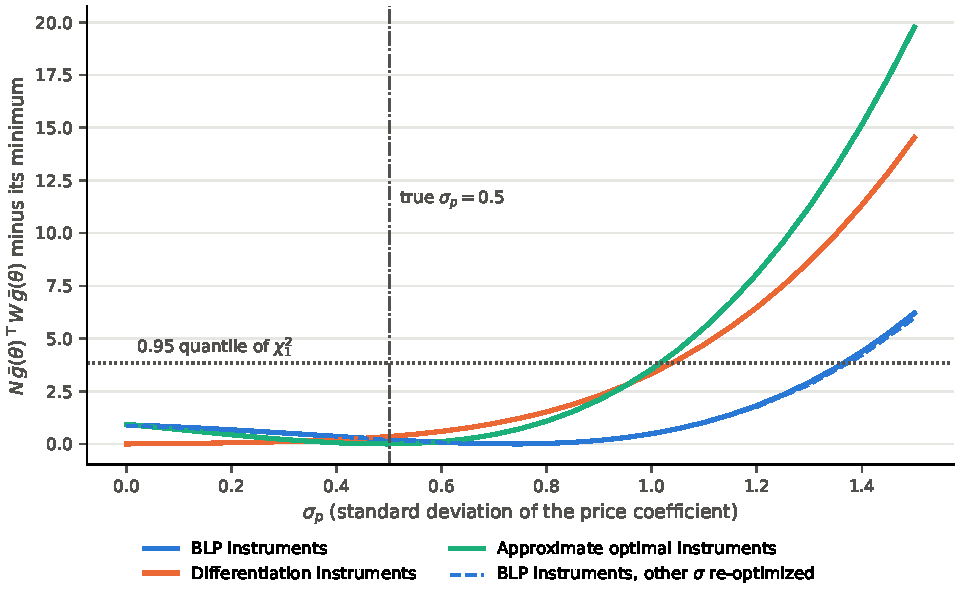
\includegraphics[width=0.92\linewidth]{figures/ch08/sim_profile.pdf}
\caption{The GMM objective as a function of the standard deviation of the price coefficient in the simulated market.
Each solid curve holds the other three standard deviations at the estimate of its instrument set, concentrates out the
linear parameters and uses the second-step weighting matrix. The dashed curve re-optimizes the other three standard
deviations for the BLP instruments. Curves are shifted so that their minimum is zero. The dotted line is the 0.95
quantile of the $\chi^2_1$ distribution, and the dash-dotted line marks the true value $\sigma_p = 0.5$.}
\label{fig:08-profile}
\end{figure}

Why is $\Sigma$ so hard to estimate here? Its identification needs variation that shifts substitution patterns
(\cref{sec:08-instruments}). In this design every product has the same characteristics and the same cost shifter in
every market. The only sources of cross-market variation are the choice set and the prices, and the price of a given
product varies little across markets. Its standard deviation across markets is between 0.045 and 0.061, against 0.189
for all prices together. The inside goods also take only 5 to 21 percent of each market, so most substitution is to
the outside good. Changes in the choice set then move the shares of the remaining products by small amounts, which the
demand shocks, with standard deviation 0.50, easily mask. The simulation correction is small by comparison. It raises
the standard errors by at most 6 percent with the BLP instruments and by less than 1 percent with the other two sets.

The lesson is general. The price coefficient is identified by the cost shifter in every specification, and its
instrumental variables estimates range from 2.5 to 3.5. The standard deviations depend on much weaker variation. A good fit and an
unrejected overidentification test do not certify them. Step 7 shows what is at stake for the substitution patterns.

\subsection{Step 7: elasticities and diversion}\label{sec:08-worked-elas}

We compute the price elasticities of market 0 under each model. Under the random coefficients models we use the
1,000 estimation draws and the recovered mean utilities of that market, and the derivatives of
\cref{prop:08-derivs}. The true elasticities use the true parameters and 200,000 draws, which approximates the
population integral. \Cref{tab:08-sim-elas} reports three objects: the own-price elasticities, the
responses of all shares to the price of product 4, and the diversion ratio to the outside good,
$-\frac{\partial s_0}{\partial p_k}\big(\frac{\partial s_k}{\partial p_k}\big)^{-1}$ (\cref{prop:08-diversion}). Own elasticities are
reported as positive numbers.

\begin{table}[htbp]
\centering
\caption{Elasticities and diversion in market 0.}
\label{tab:08-sim-elas}
\footnotesize
\begin{tabular}{lccccc}
\toprule
 & Logit & \multicolumn{3}{c}{Random coefficients logit} & True \\
\cmidrule(lr){3-5}
 & 2SLS & $\Sigma$ known & \makecell{GMM, approx.\\ optimal IV} & \makecell{GMM,\\ BLP IV} & \\
\midrule
\multicolumn{6}{l}{\emph{A. Own-price elasticity} $-\frac{\partial s_j}{\partial p_j}\frac{p_j}{s_j}$} \\
Product 2 & 3.47 & 3.45 & 3.45 & 3.78 & 3.58 \\
Product 3 & 2.62 & 2.68 & 2.67 & 3.02 & 2.76 \\
Product 4 & 3.70 & 3.63 & 3.64 & 3.42 & 3.77 \\
Product 6 & 2.59 & 2.65 & 2.64 & 2.99 & 2.74 \\
Product 8 & 2.80 & 2.79 & 2.81 & 3.12 & 2.89 \\
Product 9 & 3.81 & 3.74 & 3.74 & 4.01 & 3.87 \\
Product 10 & 2.44 & 2.51 & 2.51 & 2.85 & 2.59 \\
\addlinespace
\multicolumn{6}{l}{\emph{B. Cross-price elasticity with respect to $p_4$,} $\frac{\partial s_j}{\partial p_4}\frac{p_4}{s_j}$} \\
Product 2 & 0.047 & 0.078 & 0.063 & 0.988 & 0.069 \\
Product 3 & 0.047 & 0.067 & 0.059 & 0.038 & 0.060 \\
Product 6 & 0.047 & 0.066 & 0.059 & 0.038 & 0.059 \\
Product 8 & 0.047 & 0.069 & 0.060 & 0.039 & 0.062 \\
Product 9 & 0.047 & 0.079 & 0.064 & 0.978 & 0.070 \\
Product 10 & 0.047 & 0.066 & 0.058 & 0.038 & 0.059 \\
Outside good & 0.047 & 0.043 & 0.044 & 0.032 & 0.040 \\
\addlinespace
\multicolumn{6}{l}{\emph{C. Diversion to the outside good (percent)}} \\
Product 2 & 85.9 & 79.5 & 82.1 & 55.5 & 80.3 \\
Product 3 & 87.7 & 83.4 & 85.2 & 85.7 & 84.0 \\
Product 4 & 86.6 & 80.1 & 82.6 & 64.1 & 80.8 \\
Product 6 & 87.3 & 83.0 & 84.8 & 85.2 & 83.5 \\
Product 8 & 90.6 & 86.7 & 88.4 & 88.9 & 87.2 \\
Product 9 & 86.0 & 79.2 & 81.8 & 55.3 & 80.2 \\
Product 10 & 87.2 & 83.1 & 85.0 & 85.5 & 83.8 \\
\bottomrule
\end{tabular}
\par\smallskip
\parbox{\linewidth}{\footnotesize Notes: Market 0, at observed prices and realized shares. The columns use the
estimates of columns (2), (3), (6) and (4) of \cref{tab:08-sim-demand}. The true values use the true parameters, the
true mean utilities and 200,000 draws. Products 2, 4 and 9 are the organic products and the three most expensive.}
\end{table}

The own elasticities differ little across the logit, the random coefficients model with $\Sigma$ known and the model
estimated with approximate optimal instruments. All three are within 0.15 of the truth, and all are slightly too small
because the estimated price coefficients are below 3. The three most expensive products are the most elastic in every
column. With small shares the logit own elasticity is close to $\alpha p_j$, so this ordering is mechanical in the
logit. In the true model it also holds, because the standard deviation of the price coefficient is moderate.

The cross elasticities separate the models. In the logit, a rise in $p_4$ raises every share, including the outside
share, by the same 0.047 percent per percent. This is the IIA property of \cref{ch:logit}. In the true model the
organic products 2 and 9 gain most (0.069 and 0.070), the other products less (0.059 to 0.062), and the outside good
least (0.040). The model with $\Sigma$ known reproduces this pattern. The model estimated with approximate optimal
instruments shows it only weakly (0.063 and 0.064 against 0.058 to 0.060). Its estimate of $\sigma$ on organic is
zero, so only the random coefficient on price separates the expensive organic products. The model estimated with
BLP instruments gets the pattern badly wrong. Its large $\sigma$ on organic makes products 2 and 9 nearly perfect
substitutes for product 4, with cross elasticities of 0.988 and 0.978, about fourteen times the true values.

Diversion to the outside good tells the same story. The logit sends between 85.9 and 90.6 percent of a product's lost
buyers to the outside good, the value $\frac{s_0}{1 - s_k}$ of \cref{ch:logit}. The true model sends between 80.2 and
87.2 percent, and the models with $\Sigma$ known and with approximate optimal instruments come close. Under the BLP
instrument estimates, only 55 percent of the buyers lost by product 2 or 9 leave the market. Panel B suggests where
the others go: to the other organic products. A merger between the firms that sell products 2 and 9 would look far more harmful
under these estimates than under the true model (\cref{ch:mergers}). \Cref{fig:08-ownelas} summarizes the comparison.

\begin{figure}[htbp]
\centering
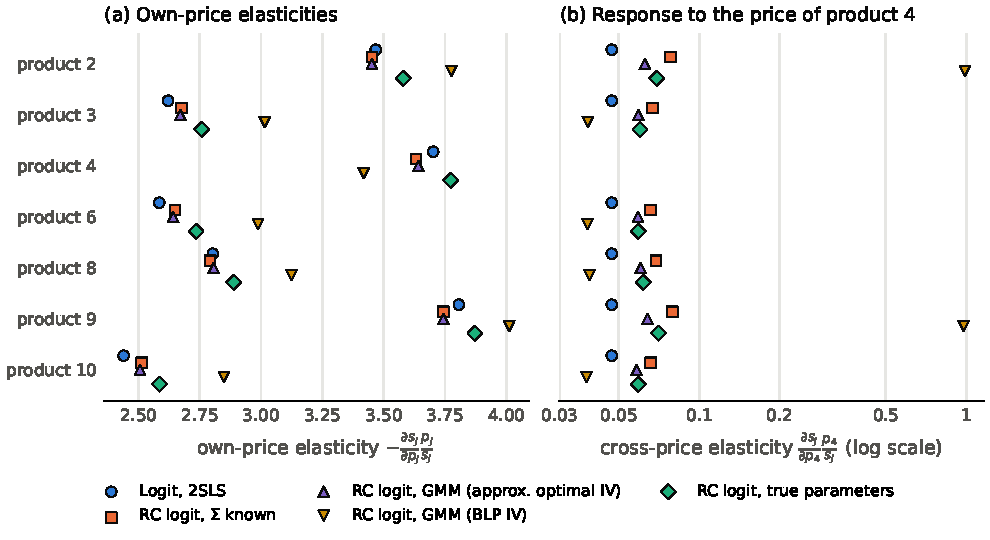
\includegraphics[width=\linewidth]{figures/ch08/sim_ownelas.pdf}
\caption{Elasticities in market 0 of the simulated market. Panel (a) shows own-price elasticities as positive numbers.
Panel (b) shows the cross-price elasticity of each product's share with respect to the price of product 4, on a log
scale. The random coefficients columns use the estimates of \cref{tab:08-sim-demand}, and the true values use 200,000
draws.}
\label{fig:08-ownelas}
\end{figure}

\subsection{What the simulated market teaches}\label{sec:08-worked-lessons}

Four lessons carry over to applications. First, the computational steps are fast and reliable when implemented
carefully. The Morrow-Skerlos iteration finds the equilibrium in 10 to 13 iterations, and the contraction recovers the
mean utilities to $10^{-12}$ in about 15 to 25 iterations. Second, a strong cost shifter identifies the mean price
coefficient well. The logit estimate is biased toward zero by the sorting of less price-sensitive consumers into
expensive products, and the random coefficients model removes most of the bias when $\Sigma$ is right.

Third, $\Sigma$ is the hard part. With market-level data its identification rests on variation in choice sets and in
the characteristics of competing products. When that variation is weak, the estimates of $\Sigma$ and the substitution
patterns they imply can be far from the truth, even when the overidentification test passes. The diagnostics that
reveal the problem are cheap: several starting values, the profile of the objective, the eigenvalues of $G^\top WG$,
and comparisons across instrument sets.

Fourth, the remedies are the subjects of the preceding sections. Richer cross-market variation helps, as do approximate
optimal instruments. Micro moments and second-choice data identify $\Sigma$ from within-market variation
(\cref{sec:08-micro}). A supply side adds moments that depend on $\Sigma$ through the markups (\cref{sec:08-supply}).
Where none of these is available, the appropriate report is the range of substitution patterns consistent with the
data.
